\documentclass[twoside]{book}

% Packages required by doxygen
\usepackage{fixltx2e}
\usepackage{calc}
\usepackage{doxygen}
\usepackage[export]{adjustbox} % also loads graphicx
\usepackage{graphicx}
\usepackage[utf8]{inputenc}
\usepackage{makeidx}
\usepackage{multicol}
\usepackage{multirow}
\PassOptionsToPackage{warn}{textcomp}
\usepackage{textcomp}
\usepackage[nointegrals]{wasysym}
\usepackage[table]{xcolor}

% Font selection
\usepackage[T1]{fontenc}
\usepackage[scaled=.90]{helvet}
\usepackage{courier}
\usepackage{amssymb}
\usepackage{sectsty}
\renewcommand{\familydefault}{\sfdefault}
\allsectionsfont{%
  \fontseries{bc}\selectfont%
  \color{darkgray}%
}
\renewcommand{\DoxyLabelFont}{%
  \fontseries{bc}\selectfont%
  \color{darkgray}%
}
\newcommand{\+}{\discretionary{\mbox{\scriptsize$\hookleftarrow$}}{}{}}

% Page & text layout
\usepackage{geometry}
\geometry{%
  a4paper,%
  top=2.5cm,%
  bottom=2.5cm,%
  left=2.5cm,%
  right=2.5cm%
}
\tolerance=750
\hfuzz=15pt
\hbadness=750
\setlength{\emergencystretch}{15pt}
\setlength{\parindent}{0cm}
\setlength{\parskip}{3ex plus 2ex minus 2ex}
\makeatletter
\renewcommand{\paragraph}{%
  \@startsection{paragraph}{4}{0ex}{-1.0ex}{1.0ex}{%
    \normalfont\normalsize\bfseries\SS@parafont%
  }%
}
\renewcommand{\subparagraph}{%
  \@startsection{subparagraph}{5}{0ex}{-1.0ex}{1.0ex}{%
    \normalfont\normalsize\bfseries\SS@subparafont%
  }%
}
\makeatother

% Headers & footers
\usepackage{fancyhdr}
\pagestyle{fancyplain}
\fancyhead[LE]{\fancyplain{}{\bfseries\thepage}}
\fancyhead[CE]{\fancyplain{}{}}
\fancyhead[RE]{\fancyplain{}{\bfseries\leftmark}}
\fancyhead[LO]{\fancyplain{}{\bfseries\rightmark}}
\fancyhead[CO]{\fancyplain{}{}}
\fancyhead[RO]{\fancyplain{}{\bfseries\thepage}}
\fancyfoot[LE]{\fancyplain{}{}}
\fancyfoot[CE]{\fancyplain{}{}}
\fancyfoot[RE]{\fancyplain{}{\bfseries\scriptsize Generated by Doxygen }}
\fancyfoot[LO]{\fancyplain{}{\bfseries\scriptsize Generated by Doxygen }}
\fancyfoot[CO]{\fancyplain{}{}}
\fancyfoot[RO]{\fancyplain{}{}}
\renewcommand{\footrulewidth}{0.4pt}
\renewcommand{\chaptermark}[1]{%
  \markboth{#1}{}%
}
\renewcommand{\sectionmark}[1]{%
  \markright{\thesection\ #1}%
}

% Indices & bibliography
\usepackage{natbib}
\usepackage[titles]{tocloft}
\setcounter{tocdepth}{3}
\setcounter{secnumdepth}{5}
\makeindex

% Hyperlinks (required, but should be loaded last)
\usepackage{ifpdf}
\ifpdf
  \usepackage[pdftex,pagebackref=true]{hyperref}
\else
  \usepackage[ps2pdf,pagebackref=true]{hyperref}
\fi
\hypersetup{%
  colorlinks=true,%
  linkcolor=blue,%
  citecolor=blue,%
  unicode%
}

% Custom commands
\newcommand{\clearemptydoublepage}{%
  \newpage{\pagestyle{empty}\cleardoublepage}%
}

\usepackage{caption}
\captionsetup{labelsep=space,justification=centering,font={bf},singlelinecheck=off,skip=4pt,position=top}

%===== C O N T E N T S =====

\begin{document}

% Titlepage & ToC
\hypersetup{pageanchor=false,
             bookmarksnumbered=true,
             pdfencoding=unicode
            }
\pagenumbering{alph}
\begin{titlepage}
\vspace*{7cm}
\begin{center}%
{\Large Data\+Tables }\\
\vspace*{1cm}
{\large Generated by Doxygen 1.8.13}\\
\end{center}
\end{titlepage}
\clearemptydoublepage
\pagenumbering{roman}
\tableofcontents
\clearemptydoublepage
\pagenumbering{arabic}
\hypersetup{pageanchor=true}

%--- Begin generated contents ---
\chapter{Namespace Index}
\section{Namespace List}
Here is a list of all documented namespaces with brief descriptions\+:\begin{DoxyCompactList}
\item\contentsline{section}{\hyperlink{namespacehamburgscleanest}{hamburgscleanest} }{\pageref{namespacehamburgscleanest}}{}
\end{DoxyCompactList}

\chapter{Hierarchical Index}
\section{Class Hierarchy}
This inheritance list is sorted roughly, but not completely, alphabetically\+:\begin{DoxyCompactList}
\item \contentsline{section}{Column}{\pageref{classhamburgscleanest_1_1_data_tables_1_1_models_1_1_column}}{}
\item \contentsline{section}{Column\+Formatter}{\pageref{interfacehamburgscleanest_1_1_data_tables_1_1_interfaces_1_1_column_formatter}}{}
\begin{DoxyCompactList}
\item \contentsline{section}{Date\+Column}{\pageref{classhamburgscleanest_1_1_data_tables_1_1_models_1_1_column_formatters_1_1_date_column}}{}
\end{DoxyCompactList}
\item \contentsline{section}{Data\+Component}{\pageref{classhamburgscleanest_1_1_data_tables_1_1_models_1_1_data_component}}{}
\begin{DoxyCompactList}
\item \contentsline{section}{Data\+Scout}{\pageref{classhamburgscleanest_1_1_data_tables_1_1_models_1_1_data_components_1_1_data_scout}}{}
\item \contentsline{section}{Paginator}{\pageref{classhamburgscleanest_1_1_data_tables_1_1_models_1_1_data_components_1_1_paginator}}{}
\item \contentsline{section}{Sorter}{\pageref{classhamburgscleanest_1_1_data_tables_1_1_models_1_1_data_components_1_1_sorter}}{}
\end{DoxyCompactList}
\item \contentsline{section}{Data\+Table}{\pageref{classhamburgscleanest_1_1_data_tables_1_1_models_1_1_data_table}}{}
\item \contentsline{section}{Header}{\pageref{classhamburgscleanest_1_1_data_tables_1_1_models_1_1_header}}{}
\item \contentsline{section}{Header\+Formatter}{\pageref{interfacehamburgscleanest_1_1_data_tables_1_1_interfaces_1_1_header_formatter}}{}
\begin{DoxyCompactList}
\item \contentsline{section}{Sortable\+Header}{\pageref{classhamburgscleanest_1_1_data_tables_1_1_models_1_1_header_formatters_1_1_sortable_header}}{}
\item \contentsline{section}{Translate\+Header}{\pageref{classhamburgscleanest_1_1_data_tables_1_1_models_1_1_header_formatters_1_1_translate_header}}{}
\end{DoxyCompactList}
\item \contentsline{section}{Relation}{\pageref{classhamburgscleanest_1_1_data_tables_1_1_models_1_1_relation}}{}
\item \contentsline{section}{Session\+Helper}{\pageref{classhamburgscleanest_1_1_data_tables_1_1_helpers_1_1_session_helper}}{}
\item \contentsline{section}{Table\+Renderer}{\pageref{classhamburgscleanest_1_1_data_tables_1_1_helpers_1_1_table_renderer}}{}
\item \contentsline{section}{Url\+Helper}{\pageref{classhamburgscleanest_1_1_data_tables_1_1_helpers_1_1_url_helper}}{}
\item Facade\begin{DoxyCompactList}
\item \contentsline{section}{Data\+Table}{\pageref{classhamburgscleanest_1_1_data_tables_1_1_facades_1_1_data_table}}{}
\item \contentsline{section}{Session\+Helper}{\pageref{classhamburgscleanest_1_1_data_tables_1_1_facades_1_1_session_helper}}{}
\item \contentsline{section}{Table\+Renderer}{\pageref{classhamburgscleanest_1_1_data_tables_1_1_facades_1_1_table_renderer}}{}
\item \contentsline{section}{Url\+Helper}{\pageref{classhamburgscleanest_1_1_data_tables_1_1_facades_1_1_url_helper}}{}
\end{DoxyCompactList}
\item Service\+Provider\begin{DoxyCompactList}
\item \contentsline{section}{Data\+Tables\+Service\+Provider}{\pageref{classhamburgscleanest_1_1_data_tables_1_1_data_tables_service_provider}}{}
\end{DoxyCompactList}
\end{DoxyCompactList}

\chapter{Data Structure Index}
\section{Data Structures}
Here are the data structures with brief descriptions\+:\begin{DoxyCompactList}
\item\contentsline{section}{\hyperlink{classhamburgscleanest_1_1_data_tables_1_1_models_1_1_column_1_1_column}{Column} }{\pageref{classhamburgscleanest_1_1_data_tables_1_1_models_1_1_column_1_1_column}}{}
\item\contentsline{section}{\hyperlink{interfacehamburgscleanest_1_1_data_tables_1_1_interfaces_1_1_column_formatter}{Column\+Formatter} }{\pageref{interfacehamburgscleanest_1_1_data_tables_1_1_interfaces_1_1_column_formatter}}{}
\item\contentsline{section}{\hyperlink{classhamburgscleanest_1_1_data_tables_1_1_models_1_1_column_1_1_column_relation}{Column\+Relation} }{\pageref{classhamburgscleanest_1_1_data_tables_1_1_models_1_1_column_1_1_column_relation}}{}
\item\contentsline{section}{\hyperlink{classhamburgscleanest_1_1_data_tables_1_1_models_1_1_data_component}{Data\+Component} }{\pageref{classhamburgscleanest_1_1_data_tables_1_1_models_1_1_data_component}}{}
\item\contentsline{section}{\hyperlink{classhamburgscleanest_1_1_data_tables_1_1_models_1_1_data_components_1_1_data_scout}{Data\+Scout} }{\pageref{classhamburgscleanest_1_1_data_tables_1_1_models_1_1_data_components_1_1_data_scout}}{}
\item\contentsline{section}{\hyperlink{classhamburgscleanest_1_1_data_tables_1_1_facades_1_1_data_table}{Data\+Table} }{\pageref{classhamburgscleanest_1_1_data_tables_1_1_facades_1_1_data_table}}{}
\item\contentsline{section}{\hyperlink{classhamburgscleanest_1_1_data_tables_1_1_models_1_1_data_table}{Data\+Table} }{\pageref{classhamburgscleanest_1_1_data_tables_1_1_models_1_1_data_table}}{}
\item\contentsline{section}{\hyperlink{classhamburgscleanest_1_1_data_tables_1_1_data_tables_service_provider}{Data\+Tables\+Service\+Provider} }{\pageref{classhamburgscleanest_1_1_data_tables_1_1_data_tables_service_provider}}{}
\item\contentsline{section}{\hyperlink{classhamburgscleanest_1_1_data_tables_1_1_models_1_1_column_formatters_1_1_date_column}{Date\+Column} }{\pageref{classhamburgscleanest_1_1_data_tables_1_1_models_1_1_column_formatters_1_1_date_column}}{}
\item\contentsline{section}{\hyperlink{classhamburgscleanest_1_1_data_tables_1_1_models_1_1_column_formatters_1_1_adapters_1_1_icon_1_1_font_awesome_adapter}{Font\+Awesome\+Adapter} }{\pageref{classhamburgscleanest_1_1_data_tables_1_1_models_1_1_column_formatters_1_1_adapters_1_1_icon_1_1_font_awesome_adapter}}{}
\item\contentsline{section}{\hyperlink{classhamburgscleanest_1_1_data_tables_1_1_models_1_1_header}{Header} }{\pageref{classhamburgscleanest_1_1_data_tables_1_1_models_1_1_header}}{}
\item\contentsline{section}{\hyperlink{interfacehamburgscleanest_1_1_data_tables_1_1_interfaces_1_1_header_formatter}{Header\+Formatter} }{\pageref{interfacehamburgscleanest_1_1_data_tables_1_1_interfaces_1_1_header_formatter}}{}
\item\contentsline{section}{\hyperlink{interfacehamburgscleanest_1_1_data_tables_1_1_models_1_1_column_formatters_1_1_adapters_1_1_icon_1_1_icon_adapter}{Icon\+Adapter} }{\pageref{interfacehamburgscleanest_1_1_data_tables_1_1_models_1_1_column_formatters_1_1_adapters_1_1_icon_1_1_icon_adapter}}{}
\item\contentsline{section}{\hyperlink{classhamburgscleanest_1_1_data_tables_1_1_models_1_1_column_formatters_1_1_icon_column}{Icon\+Column} }{\pageref{classhamburgscleanest_1_1_data_tables_1_1_models_1_1_column_formatters_1_1_icon_column}}{}
\item\contentsline{section}{\hyperlink{classhamburgscleanest_1_1_data_tables_1_1_models_1_1_column_formatters_1_1_image_column}{Image\+Column} }{\pageref{classhamburgscleanest_1_1_data_tables_1_1_models_1_1_column_formatters_1_1_image_column}}{}
\item\contentsline{section}{\hyperlink{classhamburgscleanest_1_1_data_tables_1_1_exceptions_1_1_multiple_component_assertion_exception}{Multiple\+Component\+Assertion\+Exception} }{\pageref{classhamburgscleanest_1_1_data_tables_1_1_exceptions_1_1_multiple_component_assertion_exception}}{}
\item\contentsline{section}{\hyperlink{classhamburgscleanest_1_1_data_tables_1_1_models_1_1_data_components_1_1_paginator}{Paginator} }{\pageref{classhamburgscleanest_1_1_data_tables_1_1_models_1_1_data_components_1_1_paginator}}{}
\item\contentsline{section}{\hyperlink{classhamburgscleanest_1_1_data_tables_1_1_models_1_1_relationship}{Relationship} }{\pageref{classhamburgscleanest_1_1_data_tables_1_1_models_1_1_relationship}}{}
\item\contentsline{section}{\hyperlink{classhamburgscleanest_1_1_data_tables_1_1_facades_1_1_session_helper}{Session\+Helper} }{\pageref{classhamburgscleanest_1_1_data_tables_1_1_facades_1_1_session_helper}}{}
\item\contentsline{section}{\hyperlink{classhamburgscleanest_1_1_data_tables_1_1_helpers_1_1_session_helper}{Session\+Helper} }{\pageref{classhamburgscleanest_1_1_data_tables_1_1_helpers_1_1_session_helper}}{}
\item\contentsline{section}{\hyperlink{classhamburgscleanest_1_1_data_tables_1_1_models_1_1_header_formatters_1_1_sortable_header}{Sortable\+Header} }{\pageref{classhamburgscleanest_1_1_data_tables_1_1_models_1_1_header_formatters_1_1_sortable_header}}{}
\item\contentsline{section}{\hyperlink{classhamburgscleanest_1_1_data_tables_1_1_models_1_1_data_components_1_1_sorter}{Sorter} }{\pageref{classhamburgscleanest_1_1_data_tables_1_1_models_1_1_data_components_1_1_sorter}}{}
\item\contentsline{section}{\hyperlink{classhamburgscleanest_1_1_data_tables_1_1_helpers_1_1_table_renderer}{Table\+Renderer} }{\pageref{classhamburgscleanest_1_1_data_tables_1_1_helpers_1_1_table_renderer}}{}
\item\contentsline{section}{\hyperlink{classhamburgscleanest_1_1_data_tables_1_1_facades_1_1_table_renderer}{Table\+Renderer} }{\pageref{classhamburgscleanest_1_1_data_tables_1_1_facades_1_1_table_renderer}}{}
\item\contentsline{section}{\hyperlink{classhamburgscleanest_1_1_data_tables_1_1_models_1_1_header_formatters_1_1_translate_header}{Translate\+Header} }{\pageref{classhamburgscleanest_1_1_data_tables_1_1_models_1_1_header_formatters_1_1_translate_header}}{}
\item\contentsline{section}{\hyperlink{classhamburgscleanest_1_1_data_tables_1_1_facades_1_1_url_helper}{Url\+Helper} }{\pageref{classhamburgscleanest_1_1_data_tables_1_1_facades_1_1_url_helper}}{}
\item\contentsline{section}{\hyperlink{classhamburgscleanest_1_1_data_tables_1_1_helpers_1_1_url_helper}{Url\+Helper} }{\pageref{classhamburgscleanest_1_1_data_tables_1_1_helpers_1_1_url_helper}}{}
\end{DoxyCompactList}

\chapter{Namespace Documentation}
\hypertarget{namespacehamburgscleanest}{}\section{hamburgscleanest Namespace Reference}
\label{namespacehamburgscleanest}\index{hamburgscleanest@{hamburgscleanest}}


\subsection{Detailed Description}
Class Data\+Tables\+Service\+Provider 

Class Data\+Table 

Class Session\+Helper 

Class Table\+Renderer 

Class Url\+Helper 

Class Session\+Helper 

Class Table\+Renderer 

Class Url\+Helper 

Interface Column\+Formatter 

Interface Header\+Formatter 

Class Header 

Class Date\+Column 

Class Data\+Component 

Class Data\+Scout 

Class Paginator 

Class Sorter 

Class Data\+Table 

Class Sortable\+Header

Either whitelist the headers you want to make sortable or blacklist the headers you do not want to become sortable.

If nothing is specified, all headers are sortable.

Class Translate\+Header

Class Relation  
\chapter{Data Structure Documentation}
\hypertarget{classhamburgscleanest_1_1_data_tables_1_1_models_1_1_column}{}\section{Column Class Reference}
\label{classhamburgscleanest_1_1_data_tables_1_1_models_1_1_column}\index{Column@{Column}}
\subsection*{Public Member Functions}
\begin{DoxyCompactItemize}
\item 
\hyperlink{classhamburgscleanest_1_1_data_tables_1_1_models_1_1_column_a1164c670a9c8d4167848374c2ce101cc}{\+\_\+\+\_\+construct} (string \$name, ? \hyperlink{interfacehamburgscleanest_1_1_data_tables_1_1_interfaces_1_1_column_formatter}{Column\+Formatter} \$column\+Formatter=null)
\item 
\hyperlink{classhamburgscleanest_1_1_data_tables_1_1_models_1_1_column_ad40c766ec8aced9770fe6ae269a1e781}{get\+Key} ()
\item 
\hyperlink{classhamburgscleanest_1_1_data_tables_1_1_models_1_1_column_a3d0963e68bb313b163a73f2803c64600}{get\+Name} ()
\item 
\hyperlink{classhamburgscleanest_1_1_data_tables_1_1_models_1_1_column_aef428fd06c26df985591f168f4387ddf}{get\+Attribute\+Name} ()
\item 
\hyperlink{classhamburgscleanest_1_1_data_tables_1_1_models_1_1_column_ab4da3592f01f7673fec5163a047cc82e}{get\+Relation} ()
\item 
\hyperlink{classhamburgscleanest_1_1_data_tables_1_1_models_1_1_column_ab66956c2516c8994e6965e79e73bae56}{set\+Formatter} (\hyperlink{interfacehamburgscleanest_1_1_data_tables_1_1_interfaces_1_1_column_formatter}{Column\+Formatter} \$column\+Formatter)
\item 
\hyperlink{classhamburgscleanest_1_1_data_tables_1_1_models_1_1_column_a26f5178f9badcf426408b131cb925797}{get\+Formatted\+Value} (Model \$row\+Model)
\item 
\hyperlink{classhamburgscleanest_1_1_data_tables_1_1_models_1_1_column_ae1281be756bd4669920b08da359f3dd6}{get\+Value} (Model \$row\+Model)
\end{DoxyCompactItemize}


\subsection{Constructor \& Destructor Documentation}
\mbox{\Hypertarget{classhamburgscleanest_1_1_data_tables_1_1_models_1_1_column_a1164c670a9c8d4167848374c2ce101cc}\label{classhamburgscleanest_1_1_data_tables_1_1_models_1_1_column_a1164c670a9c8d4167848374c2ce101cc}} 
\index{hamburgscleanest\+::\+Data\+Tables\+::\+Models\+::\+Column@{hamburgscleanest\+::\+Data\+Tables\+::\+Models\+::\+Column}!\+\_\+\+\_\+construct@{\+\_\+\+\_\+construct}}
\index{\+\_\+\+\_\+construct@{\+\_\+\+\_\+construct}!hamburgscleanest\+::\+Data\+Tables\+::\+Models\+::\+Column@{hamburgscleanest\+::\+Data\+Tables\+::\+Models\+::\+Column}}
\subsubsection{\texorpdfstring{\+\_\+\+\_\+construct()}{\_\_construct()}}
{\footnotesize\ttfamily \+\_\+\+\_\+construct (\begin{DoxyParamCaption}\item[{string}]{\$name,  }\item[{? \hyperlink{interfacehamburgscleanest_1_1_data_tables_1_1_interfaces_1_1_column_formatter}{Column\+Formatter}}]{\$column\+Formatter = {\ttfamily null} }\end{DoxyParamCaption})}

\hyperlink{classhamburgscleanest_1_1_data_tables_1_1_models_1_1_column}{Column} constructor. 
\begin{DoxyParams}[1]{Parameters}
string & {\em \$name} & \\
\hline
Column\+Formatter | null & {\em \$column\+Formatter} & \\
\hline
\end{DoxyParams}


\subsection{Member Function Documentation}
\mbox{\Hypertarget{classhamburgscleanest_1_1_data_tables_1_1_models_1_1_column_aef428fd06c26df985591f168f4387ddf}\label{classhamburgscleanest_1_1_data_tables_1_1_models_1_1_column_aef428fd06c26df985591f168f4387ddf}} 
\index{hamburgscleanest\+::\+Data\+Tables\+::\+Models\+::\+Column@{hamburgscleanest\+::\+Data\+Tables\+::\+Models\+::\+Column}!get\+Attribute\+Name@{get\+Attribute\+Name}}
\index{get\+Attribute\+Name@{get\+Attribute\+Name}!hamburgscleanest\+::\+Data\+Tables\+::\+Models\+::\+Column@{hamburgscleanest\+::\+Data\+Tables\+::\+Models\+::\+Column}}
\subsubsection{\texorpdfstring{get\+Attribute\+Name()}{getAttributeName()}}
{\footnotesize\ttfamily get\+Attribute\+Name (\begin{DoxyParamCaption}{ }\end{DoxyParamCaption})}

\begin{DoxyReturn}{Returns}
string 
\end{DoxyReturn}
\mbox{\Hypertarget{classhamburgscleanest_1_1_data_tables_1_1_models_1_1_column_a26f5178f9badcf426408b131cb925797}\label{classhamburgscleanest_1_1_data_tables_1_1_models_1_1_column_a26f5178f9badcf426408b131cb925797}} 
\index{hamburgscleanest\+::\+Data\+Tables\+::\+Models\+::\+Column@{hamburgscleanest\+::\+Data\+Tables\+::\+Models\+::\+Column}!get\+Formatted\+Value@{get\+Formatted\+Value}}
\index{get\+Formatted\+Value@{get\+Formatted\+Value}!hamburgscleanest\+::\+Data\+Tables\+::\+Models\+::\+Column@{hamburgscleanest\+::\+Data\+Tables\+::\+Models\+::\+Column}}
\subsubsection{\texorpdfstring{get\+Formatted\+Value()}{getFormattedValue()}}
{\footnotesize\ttfamily get\+Formatted\+Value (\begin{DoxyParamCaption}\item[{Model}]{\$row\+Model }\end{DoxyParamCaption})}

Get the formatted column value.


\begin{DoxyParams}[1]{Parameters}
Model & {\em \$row\+Model} & \\
\hline
\end{DoxyParams}
\begin{DoxyReturn}{Returns}
string 
\end{DoxyReturn}
\mbox{\Hypertarget{classhamburgscleanest_1_1_data_tables_1_1_models_1_1_column_ad40c766ec8aced9770fe6ae269a1e781}\label{classhamburgscleanest_1_1_data_tables_1_1_models_1_1_column_ad40c766ec8aced9770fe6ae269a1e781}} 
\index{hamburgscleanest\+::\+Data\+Tables\+::\+Models\+::\+Column@{hamburgscleanest\+::\+Data\+Tables\+::\+Models\+::\+Column}!get\+Key@{get\+Key}}
\index{get\+Key@{get\+Key}!hamburgscleanest\+::\+Data\+Tables\+::\+Models\+::\+Column@{hamburgscleanest\+::\+Data\+Tables\+::\+Models\+::\+Column}}
\subsubsection{\texorpdfstring{get\+Key()}{getKey()}}
{\footnotesize\ttfamily get\+Key (\begin{DoxyParamCaption}{ }\end{DoxyParamCaption})}

\begin{DoxyReturn}{Returns}
string 
\end{DoxyReturn}
\mbox{\Hypertarget{classhamburgscleanest_1_1_data_tables_1_1_models_1_1_column_a3d0963e68bb313b163a73f2803c64600}\label{classhamburgscleanest_1_1_data_tables_1_1_models_1_1_column_a3d0963e68bb313b163a73f2803c64600}} 
\index{hamburgscleanest\+::\+Data\+Tables\+::\+Models\+::\+Column@{hamburgscleanest\+::\+Data\+Tables\+::\+Models\+::\+Column}!get\+Name@{get\+Name}}
\index{get\+Name@{get\+Name}!hamburgscleanest\+::\+Data\+Tables\+::\+Models\+::\+Column@{hamburgscleanest\+::\+Data\+Tables\+::\+Models\+::\+Column}}
\subsubsection{\texorpdfstring{get\+Name()}{getName()}}
{\footnotesize\ttfamily get\+Name (\begin{DoxyParamCaption}{ }\end{DoxyParamCaption})}

\begin{DoxyReturn}{Returns}
string 
\end{DoxyReturn}
\mbox{\Hypertarget{classhamburgscleanest_1_1_data_tables_1_1_models_1_1_column_ab4da3592f01f7673fec5163a047cc82e}\label{classhamburgscleanest_1_1_data_tables_1_1_models_1_1_column_ab4da3592f01f7673fec5163a047cc82e}} 
\index{hamburgscleanest\+::\+Data\+Tables\+::\+Models\+::\+Column@{hamburgscleanest\+::\+Data\+Tables\+::\+Models\+::\+Column}!get\+Relation@{get\+Relation}}
\index{get\+Relation@{get\+Relation}!hamburgscleanest\+::\+Data\+Tables\+::\+Models\+::\+Column@{hamburgscleanest\+::\+Data\+Tables\+::\+Models\+::\+Column}}
\subsubsection{\texorpdfstring{get\+Relation()}{getRelation()}}
{\footnotesize\ttfamily get\+Relation (\begin{DoxyParamCaption}{ }\end{DoxyParamCaption})}

\begin{DoxyReturn}{Returns}
null$\vert$\+Relation 
\end{DoxyReturn}
\mbox{\Hypertarget{classhamburgscleanest_1_1_data_tables_1_1_models_1_1_column_ae1281be756bd4669920b08da359f3dd6}\label{classhamburgscleanest_1_1_data_tables_1_1_models_1_1_column_ae1281be756bd4669920b08da359f3dd6}} 
\index{hamburgscleanest\+::\+Data\+Tables\+::\+Models\+::\+Column@{hamburgscleanest\+::\+Data\+Tables\+::\+Models\+::\+Column}!get\+Value@{get\+Value}}
\index{get\+Value@{get\+Value}!hamburgscleanest\+::\+Data\+Tables\+::\+Models\+::\+Column@{hamburgscleanest\+::\+Data\+Tables\+::\+Models\+::\+Column}}
\subsubsection{\texorpdfstring{get\+Value()}{getValue()}}
{\footnotesize\ttfamily get\+Value (\begin{DoxyParamCaption}\item[{Model}]{\$row\+Model }\end{DoxyParamCaption})}

Get the value of this column for the given row.


\begin{DoxyParams}[1]{Parameters}
Model & {\em \$row\+Model} & \\
\hline
\end{DoxyParams}
\begin{DoxyReturn}{Returns}
string 
\end{DoxyReturn}
\mbox{\Hypertarget{classhamburgscleanest_1_1_data_tables_1_1_models_1_1_column_ab66956c2516c8994e6965e79e73bae56}\label{classhamburgscleanest_1_1_data_tables_1_1_models_1_1_column_ab66956c2516c8994e6965e79e73bae56}} 
\index{hamburgscleanest\+::\+Data\+Tables\+::\+Models\+::\+Column@{hamburgscleanest\+::\+Data\+Tables\+::\+Models\+::\+Column}!set\+Formatter@{set\+Formatter}}
\index{set\+Formatter@{set\+Formatter}!hamburgscleanest\+::\+Data\+Tables\+::\+Models\+::\+Column@{hamburgscleanest\+::\+Data\+Tables\+::\+Models\+::\+Column}}
\subsubsection{\texorpdfstring{set\+Formatter()}{setFormatter()}}
{\footnotesize\ttfamily set\+Formatter (\begin{DoxyParamCaption}\item[{\hyperlink{interfacehamburgscleanest_1_1_data_tables_1_1_interfaces_1_1_column_formatter}{Column\+Formatter}}]{\$column\+Formatter }\end{DoxyParamCaption})}


\begin{DoxyParams}[1]{Parameters}
Column\+Formatter & {\em \$column\+Formatter} & \\
\hline
\end{DoxyParams}
\begin{DoxyReturn}{Returns}
\hyperlink{classhamburgscleanest_1_1_data_tables_1_1_models_1_1_column}{Column} 
\end{DoxyReturn}


The documentation for this class was generated from the following file\+:\begin{DoxyCompactItemize}
\item 
C\+:/\+Users/chrom/\+\_\+\+P\+A\+G\+E\+S/\+Package\+Dev/packages/hamburgscleanest/\+Data\+Tables/src/\+Models/Column.\+php\end{DoxyCompactItemize}

\hypertarget{interfacehamburgscleanest_1_1_data_tables_1_1_interfaces_1_1_column_formatter}{}\section{Column\+Formatter Interface Reference}
\label{interfacehamburgscleanest_1_1_data_tables_1_1_interfaces_1_1_column_formatter}\index{Column\+Formatter@{Column\+Formatter}}


Inheritance diagram for Column\+Formatter\+:
\nopagebreak
\begin{figure}[H]
\begin{center}
\leavevmode
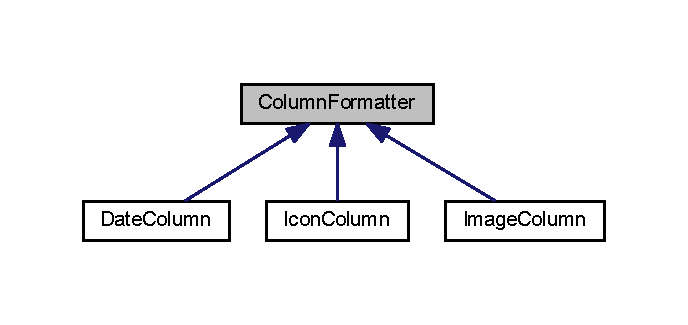
\includegraphics[width=172pt]{interfacehamburgscleanest_1_1_data_tables_1_1_interfaces_1_1_column_formatter__inherit__graph}
\end{center}
\end{figure}
\subsection*{Public Member Functions}
\begin{DoxyCompactItemize}
\item 
\hyperlink{interfacehamburgscleanest_1_1_data_tables_1_1_interfaces_1_1_column_formatter_aba259f7ae8b25e70bd444020c04606e7}{format} (string \$column)
\end{DoxyCompactItemize}


\subsection{Member Function Documentation}
\mbox{\Hypertarget{interfacehamburgscleanest_1_1_data_tables_1_1_interfaces_1_1_column_formatter_aba259f7ae8b25e70bd444020c04606e7}\label{interfacehamburgscleanest_1_1_data_tables_1_1_interfaces_1_1_column_formatter_aba259f7ae8b25e70bd444020c04606e7}} 
\index{hamburgscleanest\+::\+Data\+Tables\+::\+Interfaces\+::\+Column\+Formatter@{hamburgscleanest\+::\+Data\+Tables\+::\+Interfaces\+::\+Column\+Formatter}!format@{format}}
\index{format@{format}!hamburgscleanest\+::\+Data\+Tables\+::\+Interfaces\+::\+Column\+Formatter@{hamburgscleanest\+::\+Data\+Tables\+::\+Interfaces\+::\+Column\+Formatter}}
\subsubsection{\texorpdfstring{format()}{format()}}
{\footnotesize\ttfamily format (\begin{DoxyParamCaption}\item[{string}]{\$column }\end{DoxyParamCaption})}


\begin{DoxyParams}[1]{Parameters}
string & {\em \$column} & \\
\hline
\end{DoxyParams}
\begin{DoxyReturn}{Returns}
string 
\end{DoxyReturn}


Implemented in \hyperlink{classhamburgscleanest_1_1_data_tables_1_1_models_1_1_column_formatters_1_1_date_column_aba259f7ae8b25e70bd444020c04606e7}{Date\+Column}.



The documentation for this interface was generated from the following file\+:\begin{DoxyCompactItemize}
\item 
C\+:/\+Users/chrom/\+\_\+\+P\+A\+G\+E\+S/\+Package\+Dev/packages/hamburgscleanest/\+Data\+Tables/src/\+Interfaces/Column\+Formatter.\+php\end{DoxyCompactItemize}

\hypertarget{classhamburgscleanest_1_1_data_tables_1_1_models_1_1_data_component}{}\section{Data\+Component Class Reference}
\label{classhamburgscleanest_1_1_data_tables_1_1_models_1_1_data_component}\index{Data\+Component@{Data\+Component}}


Inheritance diagram for Data\+Component\+:\nopagebreak
\begin{figure}[H]
\begin{center}
\leavevmode
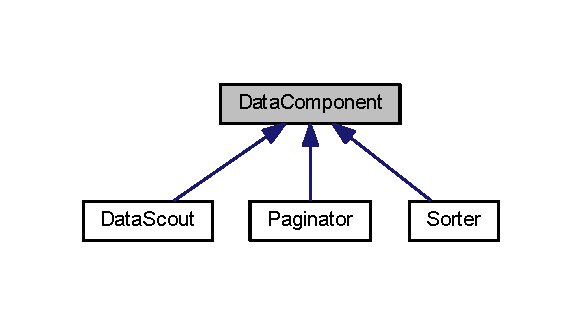
\includegraphics[width=280pt]{classhamburgscleanest_1_1_data_tables_1_1_models_1_1_data_component__inherit__graph}
\end{center}
\end{figure}
\subsection*{Public Member Functions}
\begin{DoxyCompactItemize}
\item 
\hyperlink{classhamburgscleanest_1_1_data_tables_1_1_models_1_1_data_component_a69c14abc547575170f5c45a94c58ac8a}{init} (\hyperlink{classhamburgscleanest_1_1_data_tables_1_1_models_1_1_data_table}{Data\+Table} \$data\+Table)
\item 
\hyperlink{classhamburgscleanest_1_1_data_tables_1_1_models_1_1_data_component_a565ac6563f3548952f5b3b9807799d17}{remember} ()
\item 
\hyperlink{classhamburgscleanest_1_1_data_tables_1_1_models_1_1_data_component_a5fd46320a3fc88f4322cbb025eab7cba}{forget} ()
\item 
\mbox{\Hypertarget{classhamburgscleanest_1_1_data_tables_1_1_models_1_1_data_component_a18e1ad2a8fdb81acfc1d88c1efef5f4a}\label{classhamburgscleanest_1_1_data_tables_1_1_models_1_1_data_component_a18e1ad2a8fdb81acfc1d88c1efef5f4a}} 
{\bfseries transform\+Data} ()
\item 
\hyperlink{classhamburgscleanest_1_1_data_tables_1_1_models_1_1_data_component_a3d0963e68bb313b163a73f2803c64600}{get\+Name} ()
\item 
\hyperlink{classhamburgscleanest_1_1_data_tables_1_1_models_1_1_data_component_afde88292c44dc59faf017738dae6dffb}{render} ()
\end{DoxyCompactItemize}
\subsection*{Protected Member Functions}
\begin{DoxyCompactItemize}
\item 
\hyperlink{classhamburgscleanest_1_1_data_tables_1_1_models_1_1_data_component_ae682ac7f1f1f9516c3cc2485ae5bcf4b}{\+\_\+read\+From\+Session} ()
\item 
\hyperlink{classhamburgscleanest_1_1_data_tables_1_1_models_1_1_data_component_a8b97dff3fa609aaed04b448e535ba0cc}{\+\_\+after\+Init} ()
\item 
\hyperlink{classhamburgscleanest_1_1_data_tables_1_1_models_1_1_data_component_a28881ca4bf07d4008e3ed3128198da59}{\+\_\+store\+In\+Session} ()
\item 
\hyperlink{classhamburgscleanest_1_1_data_tables_1_1_models_1_1_data_component_a6d4fda1024fd883f0750e5f0c531160d}{\+\_\+shape\+Data} ()
\end{DoxyCompactItemize}
\subsection*{Protected Attributes}
\begin{DoxyCompactItemize}
\item 
\mbox{\Hypertarget{classhamburgscleanest_1_1_data_tables_1_1_models_1_1_data_component_a57effc70e4d12c60eb1f210d9870a43b}\label{classhamburgscleanest_1_1_data_tables_1_1_models_1_1_data_component_a57effc70e4d12c60eb1f210d9870a43b}} 
{\bfseries \$\+\_\+remember\+State} = false
\item 
\mbox{\Hypertarget{classhamburgscleanest_1_1_data_tables_1_1_models_1_1_data_component_af1957828bb9ad0679ab529f6dbf639af}\label{classhamburgscleanest_1_1_data_tables_1_1_models_1_1_data_component_af1957828bb9ad0679ab529f6dbf639af}} 
{\bfseries \$\+\_\+remember\+Key} = \textquotesingle{}global\textquotesingle{}
\item 
\mbox{\Hypertarget{classhamburgscleanest_1_1_data_tables_1_1_models_1_1_data_component_a89674a8be52428c061003e413ce90575}\label{classhamburgscleanest_1_1_data_tables_1_1_models_1_1_data_component_a89674a8be52428c061003e413ce90575}} 
{\bfseries \$\+\_\+data\+Table}
\end{DoxyCompactItemize}


\subsection{Member Function Documentation}
\mbox{\Hypertarget{classhamburgscleanest_1_1_data_tables_1_1_models_1_1_data_component_a8b97dff3fa609aaed04b448e535ba0cc}\label{classhamburgscleanest_1_1_data_tables_1_1_models_1_1_data_component_a8b97dff3fa609aaed04b448e535ba0cc}} 
\index{hamburgscleanest\+::\+Data\+Tables\+::\+Models\+::\+Data\+Component@{hamburgscleanest\+::\+Data\+Tables\+::\+Models\+::\+Data\+Component}!\+\_\+after\+Init@{\+\_\+after\+Init}}
\index{\+\_\+after\+Init@{\+\_\+after\+Init}!hamburgscleanest\+::\+Data\+Tables\+::\+Models\+::\+Data\+Component@{hamburgscleanest\+::\+Data\+Tables\+::\+Models\+::\+Data\+Component}}
\subsubsection{\texorpdfstring{\+\_\+after\+Init()}{\_afterInit()}}
{\footnotesize\ttfamily \+\_\+after\+Init (\begin{DoxyParamCaption}{ }\end{DoxyParamCaption})\hspace{0.3cm}{\ttfamily [protected]}}

Initalize fields after the query builder instance is set. \mbox{\Hypertarget{classhamburgscleanest_1_1_data_tables_1_1_models_1_1_data_component_ae682ac7f1f1f9516c3cc2485ae5bcf4b}\label{classhamburgscleanest_1_1_data_tables_1_1_models_1_1_data_component_ae682ac7f1f1f9516c3cc2485ae5bcf4b}} 
\index{hamburgscleanest\+::\+Data\+Tables\+::\+Models\+::\+Data\+Component@{hamburgscleanest\+::\+Data\+Tables\+::\+Models\+::\+Data\+Component}!\+\_\+read\+From\+Session@{\+\_\+read\+From\+Session}}
\index{\+\_\+read\+From\+Session@{\+\_\+read\+From\+Session}!hamburgscleanest\+::\+Data\+Tables\+::\+Models\+::\+Data\+Component@{hamburgscleanest\+::\+Data\+Tables\+::\+Models\+::\+Data\+Component}}
\subsubsection{\texorpdfstring{\+\_\+read\+From\+Session()}{\_readFromSession()}}
{\footnotesize\ttfamily \+\_\+read\+From\+Session (\begin{DoxyParamCaption}{ }\end{DoxyParamCaption})\hspace{0.3cm}{\ttfamily [protected]}}

Everything that needs to be read when the state is remembered. Is called before \hyperlink{classhamburgscleanest_1_1_data_tables_1_1_models_1_1_data_component_a8b97dff3fa609aaed04b448e535ba0cc}{\+\_\+after\+Init()}, so that session values can be overriden. \mbox{\Hypertarget{classhamburgscleanest_1_1_data_tables_1_1_models_1_1_data_component_a6d4fda1024fd883f0750e5f0c531160d}\label{classhamburgscleanest_1_1_data_tables_1_1_models_1_1_data_component_a6d4fda1024fd883f0750e5f0c531160d}} 
\index{hamburgscleanest\+::\+Data\+Tables\+::\+Models\+::\+Data\+Component@{hamburgscleanest\+::\+Data\+Tables\+::\+Models\+::\+Data\+Component}!\+\_\+shape\+Data@{\+\_\+shape\+Data}}
\index{\+\_\+shape\+Data@{\+\_\+shape\+Data}!hamburgscleanest\+::\+Data\+Tables\+::\+Models\+::\+Data\+Component@{hamburgscleanest\+::\+Data\+Tables\+::\+Models\+::\+Data\+Component}}
\subsubsection{\texorpdfstring{\+\_\+shape\+Data()}{\_shapeData()}}
{\footnotesize\ttfamily \+\_\+shape\+Data (\begin{DoxyParamCaption}{ }\end{DoxyParamCaption})\hspace{0.3cm}{\ttfamily [abstract]}, {\ttfamily [protected]}}

\begin{DoxyReturn}{Returns}
Builder 
\end{DoxyReturn}
\mbox{\Hypertarget{classhamburgscleanest_1_1_data_tables_1_1_models_1_1_data_component_a28881ca4bf07d4008e3ed3128198da59}\label{classhamburgscleanest_1_1_data_tables_1_1_models_1_1_data_component_a28881ca4bf07d4008e3ed3128198da59}} 
\index{hamburgscleanest\+::\+Data\+Tables\+::\+Models\+::\+Data\+Component@{hamburgscleanest\+::\+Data\+Tables\+::\+Models\+::\+Data\+Component}!\+\_\+store\+In\+Session@{\+\_\+store\+In\+Session}}
\index{\+\_\+store\+In\+Session@{\+\_\+store\+In\+Session}!hamburgscleanest\+::\+Data\+Tables\+::\+Models\+::\+Data\+Component@{hamburgscleanest\+::\+Data\+Tables\+::\+Models\+::\+Data\+Component}}
\subsubsection{\texorpdfstring{\+\_\+store\+In\+Session()}{\_storeInSession()}}
{\footnotesize\ttfamily \+\_\+store\+In\+Session (\begin{DoxyParamCaption}{ }\end{DoxyParamCaption})\hspace{0.3cm}{\ttfamily [protected]}}

Use this function to save your state in the session. This is called just before rendering, so all dynamically added stuff etc. is considered. \mbox{\Hypertarget{classhamburgscleanest_1_1_data_tables_1_1_models_1_1_data_component_a5fd46320a3fc88f4322cbb025eab7cba}\label{classhamburgscleanest_1_1_data_tables_1_1_models_1_1_data_component_a5fd46320a3fc88f4322cbb025eab7cba}} 
\index{hamburgscleanest\+::\+Data\+Tables\+::\+Models\+::\+Data\+Component@{hamburgscleanest\+::\+Data\+Tables\+::\+Models\+::\+Data\+Component}!forget@{forget}}
\index{forget@{forget}!hamburgscleanest\+::\+Data\+Tables\+::\+Models\+::\+Data\+Component@{hamburgscleanest\+::\+Data\+Tables\+::\+Models\+::\+Data\+Component}}
\subsubsection{\texorpdfstring{forget()}{forget()}}
{\footnotesize\ttfamily forget (\begin{DoxyParamCaption}{ }\end{DoxyParamCaption})}

Forget the state of the data component.

\begin{DoxyReturn}{Returns}
\hyperlink{classhamburgscleanest_1_1_data_tables_1_1_models_1_1_data_component}{Data\+Component} 
\end{DoxyReturn}
\mbox{\Hypertarget{classhamburgscleanest_1_1_data_tables_1_1_models_1_1_data_component_a3d0963e68bb313b163a73f2803c64600}\label{classhamburgscleanest_1_1_data_tables_1_1_models_1_1_data_component_a3d0963e68bb313b163a73f2803c64600}} 
\index{hamburgscleanest\+::\+Data\+Tables\+::\+Models\+::\+Data\+Component@{hamburgscleanest\+::\+Data\+Tables\+::\+Models\+::\+Data\+Component}!get\+Name@{get\+Name}}
\index{get\+Name@{get\+Name}!hamburgscleanest\+::\+Data\+Tables\+::\+Models\+::\+Data\+Component@{hamburgscleanest\+::\+Data\+Tables\+::\+Models\+::\+Data\+Component}}
\subsubsection{\texorpdfstring{get\+Name()}{getName()}}
{\footnotesize\ttfamily get\+Name (\begin{DoxyParamCaption}{ }\end{DoxyParamCaption})}

\begin{DoxyReturn}{Returns}
string 
\end{DoxyReturn}
\mbox{\Hypertarget{classhamburgscleanest_1_1_data_tables_1_1_models_1_1_data_component_a69c14abc547575170f5c45a94c58ac8a}\label{classhamburgscleanest_1_1_data_tables_1_1_models_1_1_data_component_a69c14abc547575170f5c45a94c58ac8a}} 
\index{hamburgscleanest\+::\+Data\+Tables\+::\+Models\+::\+Data\+Component@{hamburgscleanest\+::\+Data\+Tables\+::\+Models\+::\+Data\+Component}!init@{init}}
\index{init@{init}!hamburgscleanest\+::\+Data\+Tables\+::\+Models\+::\+Data\+Component@{hamburgscleanest\+::\+Data\+Tables\+::\+Models\+::\+Data\+Component}}
\subsubsection{\texorpdfstring{init()}{init()}}
{\footnotesize\ttfamily init (\begin{DoxyParamCaption}\item[{\hyperlink{classhamburgscleanest_1_1_data_tables_1_1_models_1_1_data_table}{Data\+Table}}]{\$data\+Table }\end{DoxyParamCaption})}


\begin{DoxyParams}[1]{Parameters}
\hyperlink{classhamburgscleanest_1_1_data_tables_1_1_models_1_1_data_table}{Data\+Table} & {\em \$data\+Table} & \\
\hline
\end{DoxyParams}
\begin{DoxyReturn}{Returns}
\hyperlink{classhamburgscleanest_1_1_data_tables_1_1_models_1_1_data_component}{Data\+Component} 
\end{DoxyReturn}
\mbox{\Hypertarget{classhamburgscleanest_1_1_data_tables_1_1_models_1_1_data_component_a565ac6563f3548952f5b3b9807799d17}\label{classhamburgscleanest_1_1_data_tables_1_1_models_1_1_data_component_a565ac6563f3548952f5b3b9807799d17}} 
\index{hamburgscleanest\+::\+Data\+Tables\+::\+Models\+::\+Data\+Component@{hamburgscleanest\+::\+Data\+Tables\+::\+Models\+::\+Data\+Component}!remember@{remember}}
\index{remember@{remember}!hamburgscleanest\+::\+Data\+Tables\+::\+Models\+::\+Data\+Component@{hamburgscleanest\+::\+Data\+Tables\+::\+Models\+::\+Data\+Component}}
\subsubsection{\texorpdfstring{remember()}{remember()}}
{\footnotesize\ttfamily remember (\begin{DoxyParamCaption}{ }\end{DoxyParamCaption})}

Remember the state of the data component.

\begin{DoxyReturn}{Returns}
\hyperlink{classhamburgscleanest_1_1_data_tables_1_1_models_1_1_data_component}{Data\+Component} 
\end{DoxyReturn}
\mbox{\Hypertarget{classhamburgscleanest_1_1_data_tables_1_1_models_1_1_data_component_afde88292c44dc59faf017738dae6dffb}\label{classhamburgscleanest_1_1_data_tables_1_1_models_1_1_data_component_afde88292c44dc59faf017738dae6dffb}} 
\index{hamburgscleanest\+::\+Data\+Tables\+::\+Models\+::\+Data\+Component@{hamburgscleanest\+::\+Data\+Tables\+::\+Models\+::\+Data\+Component}!render@{render}}
\index{render@{render}!hamburgscleanest\+::\+Data\+Tables\+::\+Models\+::\+Data\+Component@{hamburgscleanest\+::\+Data\+Tables\+::\+Models\+::\+Data\+Component}}
\subsubsection{\texorpdfstring{render()}{render()}}
{\footnotesize\ttfamily render (\begin{DoxyParamCaption}{ }\end{DoxyParamCaption})\hspace{0.3cm}{\ttfamily [abstract]}}

\begin{DoxyReturn}{Returns}
string 
\end{DoxyReturn}


The documentation for this class was generated from the following file\+:\begin{DoxyCompactItemize}
\item 
C\+:/\+Users/chrom/\+\_\+\+P\+A\+G\+E\+S/\+Package\+Dev/packages/hamburgscleanest/\+Data\+Tables/src/\+Models/Data\+Component.\+php\end{DoxyCompactItemize}

\hypertarget{classhamburgscleanest_1_1_data_tables_1_1_models_1_1_data_components_1_1_data_scout}{}\section{Data\+Scout Class Reference}
\label{classhamburgscleanest_1_1_data_tables_1_1_models_1_1_data_components_1_1_data_scout}\index{Data\+Scout@{Data\+Scout}}


Inheritance diagram for Data\+Scout\+:\nopagebreak
\begin{figure}[H]
\begin{center}
\leavevmode
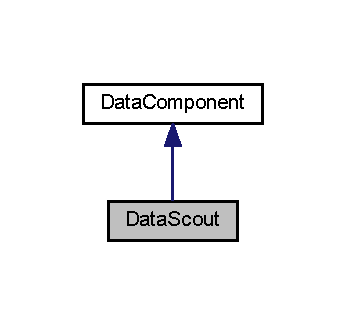
\includegraphics[width=166pt]{classhamburgscleanest_1_1_data_tables_1_1_models_1_1_data_components_1_1_data_scout__inherit__graph}
\end{center}
\end{figure}


Collaboration diagram for Data\+Scout\+:\nopagebreak
\begin{figure}[H]
\begin{center}
\leavevmode
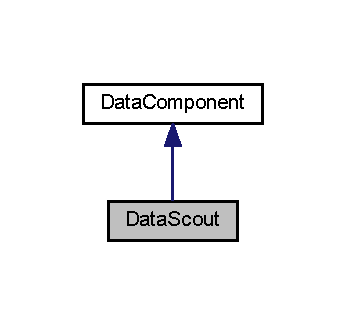
\includegraphics[width=166pt]{classhamburgscleanest_1_1_data_tables_1_1_models_1_1_data_components_1_1_data_scout__coll__graph}
\end{center}
\end{figure}
\subsection*{Public Member Functions}
\begin{DoxyCompactItemize}
\item 
\hyperlink{classhamburgscleanest_1_1_data_tables_1_1_models_1_1_data_components_1_1_data_scout_a4df8c4487c6a066c0748c13e1b986e75}{\+\_\+\+\_\+construct} (array \$searchable\+Fields=\mbox{[}$\,$\mbox{]}, \$\hyperlink{classhamburgscleanest_1_1_data_tables_1_1_models_1_1_data_component_a565ac6563f3548952f5b3b9807799d17}{remember}=false)
\item 
\hyperlink{classhamburgscleanest_1_1_data_tables_1_1_models_1_1_data_components_1_1_data_scout_a6d4fda1024fd883f0750e5f0c531160d}{\+\_\+shape\+Data} ()
\item 
\hyperlink{classhamburgscleanest_1_1_data_tables_1_1_models_1_1_data_components_1_1_data_scout_ad7dba2ef84f122056dce30d452f0e322}{add\+Query} (string \$value)
\item 
\hyperlink{classhamburgscleanest_1_1_data_tables_1_1_models_1_1_data_components_1_1_data_scout_a22411300faae3d9467b9ac2e9be16251}{button\+Text} (string \$text)
\item 
\hyperlink{classhamburgscleanest_1_1_data_tables_1_1_models_1_1_data_components_1_1_data_scout_a51d7d08dff5febd430219ac2642d6935}{placeholder} (string \$text)
\item 
\hyperlink{classhamburgscleanest_1_1_data_tables_1_1_models_1_1_data_components_1_1_data_scout_a24951165ffdc4b878efb2cc17748dea7}{make\+Searchable} (string \$field)
\item 
\hyperlink{classhamburgscleanest_1_1_data_tables_1_1_models_1_1_data_components_1_1_data_scout_afde88292c44dc59faf017738dae6dffb}{render} ()
\end{DoxyCompactItemize}
\subsection*{Protected Member Functions}
\begin{DoxyCompactItemize}
\item 
\mbox{\Hypertarget{classhamburgscleanest_1_1_data_tables_1_1_models_1_1_data_components_1_1_data_scout_a8b97dff3fa609aaed04b448e535ba0cc}\label{classhamburgscleanest_1_1_data_tables_1_1_models_1_1_data_components_1_1_data_scout_a8b97dff3fa609aaed04b448e535ba0cc}} 
{\bfseries \+\_\+after\+Init} ()
\end{DoxyCompactItemize}
\subsection*{Additional Inherited Members}


\subsection{Constructor \& Destructor Documentation}
\mbox{\Hypertarget{classhamburgscleanest_1_1_data_tables_1_1_models_1_1_data_components_1_1_data_scout_a4df8c4487c6a066c0748c13e1b986e75}\label{classhamburgscleanest_1_1_data_tables_1_1_models_1_1_data_components_1_1_data_scout_a4df8c4487c6a066c0748c13e1b986e75}} 
\index{hamburgscleanest\+::\+Data\+Tables\+::\+Models\+::\+Data\+Components\+::\+Data\+Scout@{hamburgscleanest\+::\+Data\+Tables\+::\+Models\+::\+Data\+Components\+::\+Data\+Scout}!\+\_\+\+\_\+construct@{\+\_\+\+\_\+construct}}
\index{\+\_\+\+\_\+construct@{\+\_\+\+\_\+construct}!hamburgscleanest\+::\+Data\+Tables\+::\+Models\+::\+Data\+Components\+::\+Data\+Scout@{hamburgscleanest\+::\+Data\+Tables\+::\+Models\+::\+Data\+Components\+::\+Data\+Scout}}
\subsubsection{\texorpdfstring{\+\_\+\+\_\+construct()}{\_\_construct()}}
{\footnotesize\ttfamily \+\_\+\+\_\+construct (\begin{DoxyParamCaption}\item[{array}]{\$searchable\+Fields = {\ttfamily \mbox{[}\mbox{]}},  }\item[{}]{\$remember = {\ttfamily false} }\end{DoxyParamCaption})}

\hyperlink{classhamburgscleanest_1_1_data_tables_1_1_models_1_1_data_components_1_1_data_scout}{Data\+Scout} constructor. 
\begin{DoxyParams}[1]{Parameters}
array & {\em \$searchable\+Fields} & \\
\hline
bool & {\em \$remember} & \\
\hline
\end{DoxyParams}


\subsection{Member Function Documentation}
\mbox{\Hypertarget{classhamburgscleanest_1_1_data_tables_1_1_models_1_1_data_components_1_1_data_scout_a6d4fda1024fd883f0750e5f0c531160d}\label{classhamburgscleanest_1_1_data_tables_1_1_models_1_1_data_components_1_1_data_scout_a6d4fda1024fd883f0750e5f0c531160d}} 
\index{hamburgscleanest\+::\+Data\+Tables\+::\+Models\+::\+Data\+Components\+::\+Data\+Scout@{hamburgscleanest\+::\+Data\+Tables\+::\+Models\+::\+Data\+Components\+::\+Data\+Scout}!\+\_\+shape\+Data@{\+\_\+shape\+Data}}
\index{\+\_\+shape\+Data@{\+\_\+shape\+Data}!hamburgscleanest\+::\+Data\+Tables\+::\+Models\+::\+Data\+Components\+::\+Data\+Scout@{hamburgscleanest\+::\+Data\+Tables\+::\+Models\+::\+Data\+Components\+::\+Data\+Scout}}
\subsubsection{\texorpdfstring{\+\_\+shape\+Data()}{\_shapeData()}}
{\footnotesize\ttfamily \+\_\+shape\+Data (\begin{DoxyParamCaption}{ }\end{DoxyParamCaption})}

\begin{DoxyReturn}{Returns}
Builder 
\end{DoxyReturn}
\mbox{\Hypertarget{classhamburgscleanest_1_1_data_tables_1_1_models_1_1_data_components_1_1_data_scout_ad7dba2ef84f122056dce30d452f0e322}\label{classhamburgscleanest_1_1_data_tables_1_1_models_1_1_data_components_1_1_data_scout_ad7dba2ef84f122056dce30d452f0e322}} 
\index{hamburgscleanest\+::\+Data\+Tables\+::\+Models\+::\+Data\+Components\+::\+Data\+Scout@{hamburgscleanest\+::\+Data\+Tables\+::\+Models\+::\+Data\+Components\+::\+Data\+Scout}!add\+Query@{add\+Query}}
\index{add\+Query@{add\+Query}!hamburgscleanest\+::\+Data\+Tables\+::\+Models\+::\+Data\+Components\+::\+Data\+Scout@{hamburgscleanest\+::\+Data\+Tables\+::\+Models\+::\+Data\+Components\+::\+Data\+Scout}}
\subsubsection{\texorpdfstring{add\+Query()}{addQuery()}}
{\footnotesize\ttfamily add\+Query (\begin{DoxyParamCaption}\item[{string}]{\$value }\end{DoxyParamCaption})}

Add a query programmatically.


\begin{DoxyParams}[1]{Parameters}
string & {\em \$value} & \\
\hline
\end{DoxyParams}
\begin{DoxyReturn}{Returns}
\hyperlink{classhamburgscleanest_1_1_data_tables_1_1_models_1_1_data_components_1_1_data_scout}{Data\+Scout} 
\end{DoxyReturn}
\mbox{\Hypertarget{classhamburgscleanest_1_1_data_tables_1_1_models_1_1_data_components_1_1_data_scout_a22411300faae3d9467b9ac2e9be16251}\label{classhamburgscleanest_1_1_data_tables_1_1_models_1_1_data_components_1_1_data_scout_a22411300faae3d9467b9ac2e9be16251}} 
\index{hamburgscleanest\+::\+Data\+Tables\+::\+Models\+::\+Data\+Components\+::\+Data\+Scout@{hamburgscleanest\+::\+Data\+Tables\+::\+Models\+::\+Data\+Components\+::\+Data\+Scout}!button\+Text@{button\+Text}}
\index{button\+Text@{button\+Text}!hamburgscleanest\+::\+Data\+Tables\+::\+Models\+::\+Data\+Components\+::\+Data\+Scout@{hamburgscleanest\+::\+Data\+Tables\+::\+Models\+::\+Data\+Components\+::\+Data\+Scout}}
\subsubsection{\texorpdfstring{button\+Text()}{buttonText()}}
{\footnotesize\ttfamily button\+Text (\begin{DoxyParamCaption}\item[{string}]{\$text }\end{DoxyParamCaption})}

Set the text for the search button.


\begin{DoxyParams}[1]{Parameters}
string & {\em \$text} & \\
\hline
\end{DoxyParams}
\begin{DoxyReturn}{Returns}
\hyperlink{classhamburgscleanest_1_1_data_tables_1_1_models_1_1_data_components_1_1_data_scout}{Data\+Scout} 
\end{DoxyReturn}
\mbox{\Hypertarget{classhamburgscleanest_1_1_data_tables_1_1_models_1_1_data_components_1_1_data_scout_a24951165ffdc4b878efb2cc17748dea7}\label{classhamburgscleanest_1_1_data_tables_1_1_models_1_1_data_components_1_1_data_scout_a24951165ffdc4b878efb2cc17748dea7}} 
\index{hamburgscleanest\+::\+Data\+Tables\+::\+Models\+::\+Data\+Components\+::\+Data\+Scout@{hamburgscleanest\+::\+Data\+Tables\+::\+Models\+::\+Data\+Components\+::\+Data\+Scout}!make\+Searchable@{make\+Searchable}}
\index{make\+Searchable@{make\+Searchable}!hamburgscleanest\+::\+Data\+Tables\+::\+Models\+::\+Data\+Components\+::\+Data\+Scout@{hamburgscleanest\+::\+Data\+Tables\+::\+Models\+::\+Data\+Components\+::\+Data\+Scout}}
\subsubsection{\texorpdfstring{make\+Searchable()}{makeSearchable()}}
{\footnotesize\ttfamily make\+Searchable (\begin{DoxyParamCaption}\item[{string}]{\$field }\end{DoxyParamCaption})}

Make the field searchable.


\begin{DoxyParams}[1]{Parameters}
string & {\em \$field} & \\
\hline
\end{DoxyParams}
\begin{DoxyReturn}{Returns}
\hyperlink{classhamburgscleanest_1_1_data_tables_1_1_models_1_1_data_components_1_1_data_scout}{Data\+Scout} 
\end{DoxyReturn}
\mbox{\Hypertarget{classhamburgscleanest_1_1_data_tables_1_1_models_1_1_data_components_1_1_data_scout_a51d7d08dff5febd430219ac2642d6935}\label{classhamburgscleanest_1_1_data_tables_1_1_models_1_1_data_components_1_1_data_scout_a51d7d08dff5febd430219ac2642d6935}} 
\index{hamburgscleanest\+::\+Data\+Tables\+::\+Models\+::\+Data\+Components\+::\+Data\+Scout@{hamburgscleanest\+::\+Data\+Tables\+::\+Models\+::\+Data\+Components\+::\+Data\+Scout}!placeholder@{placeholder}}
\index{placeholder@{placeholder}!hamburgscleanest\+::\+Data\+Tables\+::\+Models\+::\+Data\+Components\+::\+Data\+Scout@{hamburgscleanest\+::\+Data\+Tables\+::\+Models\+::\+Data\+Components\+::\+Data\+Scout}}
\subsubsection{\texorpdfstring{placeholder()}{placeholder()}}
{\footnotesize\ttfamily placeholder (\begin{DoxyParamCaption}\item[{string}]{\$text }\end{DoxyParamCaption})}

Set the placeholder for the input.


\begin{DoxyParams}[1]{Parameters}
string & {\em \$text} & \\
\hline
\end{DoxyParams}
\begin{DoxyReturn}{Returns}
\hyperlink{classhamburgscleanest_1_1_data_tables_1_1_models_1_1_data_components_1_1_data_scout}{Data\+Scout} 
\end{DoxyReturn}
\mbox{\Hypertarget{classhamburgscleanest_1_1_data_tables_1_1_models_1_1_data_components_1_1_data_scout_afde88292c44dc59faf017738dae6dffb}\label{classhamburgscleanest_1_1_data_tables_1_1_models_1_1_data_components_1_1_data_scout_afde88292c44dc59faf017738dae6dffb}} 
\index{hamburgscleanest\+::\+Data\+Tables\+::\+Models\+::\+Data\+Components\+::\+Data\+Scout@{hamburgscleanest\+::\+Data\+Tables\+::\+Models\+::\+Data\+Components\+::\+Data\+Scout}!render@{render}}
\index{render@{render}!hamburgscleanest\+::\+Data\+Tables\+::\+Models\+::\+Data\+Components\+::\+Data\+Scout@{hamburgscleanest\+::\+Data\+Tables\+::\+Models\+::\+Data\+Components\+::\+Data\+Scout}}
\subsubsection{\texorpdfstring{render()}{render()}}
{\footnotesize\ttfamily render (\begin{DoxyParamCaption}{ }\end{DoxyParamCaption})}

\begin{DoxyReturn}{Returns}
string 
\end{DoxyReturn}


The documentation for this class was generated from the following file\+:\begin{DoxyCompactItemize}
\item 
C\+:/\+Users/chrom/\+\_\+\+P\+A\+G\+E\+S/\+Package\+Dev/packages/hamburgscleanest/\+Data\+Tables/src/\+Models/\+Data\+Components/Data\+Scout.\+php\end{DoxyCompactItemize}

\hypertarget{classhamburgscleanest_1_1_data_tables_1_1_models_1_1_data_table}{}\section{Data\+Table Class Reference}
\label{classhamburgscleanest_1_1_data_tables_1_1_models_1_1_data_table}\index{Data\+Table@{Data\+Table}}
\subsection*{Public Member Functions}
\begin{DoxyCompactItemize}
\item 
\hyperlink{classhamburgscleanest_1_1_data_tables_1_1_models_1_1_data_table_aed2405fdf602895cf021ddf2de67f37c}{model} (string \$model\+Name, array \$\hyperlink{classhamburgscleanest_1_1_data_tables_1_1_models_1_1_data_table_aa58d366fa31ae19686c78817af00407c}{columns}=\mbox{[}$\,$\mbox{]})
\item 
\hyperlink{classhamburgscleanest_1_1_data_tables_1_1_models_1_1_data_table_a6287262cb9628d7a89d8fc16dcb51177}{get\+Columns} ()
\item 
\hyperlink{classhamburgscleanest_1_1_data_tables_1_1_models_1_1_data_table_a8dbd35d765e8ff0d1c34461ef67c5abf}{query} ()
\item 
\hyperlink{classhamburgscleanest_1_1_data_tables_1_1_models_1_1_data_table_aa58d366fa31ae19686c78817af00407c}{columns} (array \$columns)
\item 
\hyperlink{classhamburgscleanest_1_1_data_tables_1_1_models_1_1_data_table_a267226c73f5cd89ec9f01776aab256c5}{add\+Component} (\hyperlink{classhamburgscleanest_1_1_data_tables_1_1_models_1_1_data_component}{Data\+Component} \$component, ? string \$name=null)
\item 
\hyperlink{classhamburgscleanest_1_1_data_tables_1_1_models_1_1_data_table_a7b7268aff8cff85372212b29c5cdf7c5}{component\+Exists} (string \$component\+Name)
\item 
\hyperlink{classhamburgscleanest_1_1_data_tables_1_1_models_1_1_data_table_ab215f578c0cd2a411123b4878fa8fa55}{format\+Headers} (\hyperlink{interfacehamburgscleanest_1_1_data_tables_1_1_interfaces_1_1_header_formatter}{Header\+Formatter} \$header\+Formatter)
\item 
\hyperlink{classhamburgscleanest_1_1_data_tables_1_1_models_1_1_data_table_a813e5943086af6dacdea0ffc17b284d6}{classes} (string \$classes)
\item 
\hyperlink{classhamburgscleanest_1_1_data_tables_1_1_models_1_1_data_table_a27b8523da3acb9865571844d5487f6a0}{with} (array \$relations)
\item 
\hyperlink{classhamburgscleanest_1_1_data_tables_1_1_models_1_1_data_table_a82b20d38c42a9e462cdfe91b77b805a7}{no\+Data\+Html} (string \$html)
\item 
\hyperlink{classhamburgscleanest_1_1_data_tables_1_1_models_1_1_data_table_a3983a155c93b691cd1e069a3e46baaf6}{no\+Data\+View} (string \$view\+Name)
\item 
\hyperlink{classhamburgscleanest_1_1_data_tables_1_1_models_1_1_data_table_afde88292c44dc59faf017738dae6dffb}{render} ()
\item 
\hyperlink{classhamburgscleanest_1_1_data_tables_1_1_models_1_1_data_table_abc8e9e31bb15c8a44c3210ec551407c8}{\+\_\+\+\_\+get} (\$name)
\end{DoxyCompactItemize}


\subsection{Member Function Documentation}
\mbox{\Hypertarget{classhamburgscleanest_1_1_data_tables_1_1_models_1_1_data_table_abc8e9e31bb15c8a44c3210ec551407c8}\label{classhamburgscleanest_1_1_data_tables_1_1_models_1_1_data_table_abc8e9e31bb15c8a44c3210ec551407c8}} 
\index{hamburgscleanest\+::\+Data\+Tables\+::\+Models\+::\+Data\+Table@{hamburgscleanest\+::\+Data\+Tables\+::\+Models\+::\+Data\+Table}!\+\_\+\+\_\+get@{\+\_\+\+\_\+get}}
\index{\+\_\+\+\_\+get@{\+\_\+\+\_\+get}!hamburgscleanest\+::\+Data\+Tables\+::\+Models\+::\+Data\+Table@{hamburgscleanest\+::\+Data\+Tables\+::\+Models\+::\+Data\+Table}}
\subsubsection{\texorpdfstring{\+\_\+\+\_\+get()}{\_\_get()}}
{\footnotesize\ttfamily \+\_\+\+\_\+get (\begin{DoxyParamCaption}\item[{}]{\$name }\end{DoxyParamCaption})}


\begin{DoxyParams}{Parameters}
{\em \$name} & \\
\hline
\end{DoxyParams}
\begin{DoxyReturn}{Returns}
mixed 
\end{DoxyReturn}
\mbox{\Hypertarget{classhamburgscleanest_1_1_data_tables_1_1_models_1_1_data_table_a267226c73f5cd89ec9f01776aab256c5}\label{classhamburgscleanest_1_1_data_tables_1_1_models_1_1_data_table_a267226c73f5cd89ec9f01776aab256c5}} 
\index{hamburgscleanest\+::\+Data\+Tables\+::\+Models\+::\+Data\+Table@{hamburgscleanest\+::\+Data\+Tables\+::\+Models\+::\+Data\+Table}!add\+Component@{add\+Component}}
\index{add\+Component@{add\+Component}!hamburgscleanest\+::\+Data\+Tables\+::\+Models\+::\+Data\+Table@{hamburgscleanest\+::\+Data\+Tables\+::\+Models\+::\+Data\+Table}}
\subsubsection{\texorpdfstring{add\+Component()}{addComponent()}}
{\footnotesize\ttfamily add\+Component (\begin{DoxyParamCaption}\item[{\hyperlink{classhamburgscleanest_1_1_data_tables_1_1_models_1_1_data_component}{Data\+Component}}]{\$component,  }\item[{? string}]{\$name = {\ttfamily null} }\end{DoxyParamCaption})}

Add a component to the data table. For example a \char`\"{}\+Paginator\char`\"{} or a \char`\"{}\+Sorter\char`\"{}.


\begin{DoxyParams}[1]{Parameters}
\hyperlink{classhamburgscleanest_1_1_data_tables_1_1_models_1_1_data_component}{Data\+Component} & {\em \$component} & \\
\hline
null | string & {\em \$name} & \\
\hline
\end{DoxyParams}
\begin{DoxyReturn}{Returns}
\hyperlink{classhamburgscleanest_1_1_data_tables_1_1_models_1_1_data_table}{Data\+Table} 
\end{DoxyReturn}

\begin{DoxyExceptions}{Exceptions}
{\em } & \\
\hline
\end{DoxyExceptions}
\mbox{\Hypertarget{classhamburgscleanest_1_1_data_tables_1_1_models_1_1_data_table_a813e5943086af6dacdea0ffc17b284d6}\label{classhamburgscleanest_1_1_data_tables_1_1_models_1_1_data_table_a813e5943086af6dacdea0ffc17b284d6}} 
\index{hamburgscleanest\+::\+Data\+Tables\+::\+Models\+::\+Data\+Table@{hamburgscleanest\+::\+Data\+Tables\+::\+Models\+::\+Data\+Table}!classes@{classes}}
\index{classes@{classes}!hamburgscleanest\+::\+Data\+Tables\+::\+Models\+::\+Data\+Table@{hamburgscleanest\+::\+Data\+Tables\+::\+Models\+::\+Data\+Table}}
\subsubsection{\texorpdfstring{classes()}{classes()}}
{\footnotesize\ttfamily classes (\begin{DoxyParamCaption}\item[{string}]{\$classes }\end{DoxyParamCaption})}

Add classes to the table.


\begin{DoxyParams}[1]{Parameters}
string & {\em \$classes} & \\
\hline
\end{DoxyParams}
\begin{DoxyReturn}{Returns}
\$this 
\end{DoxyReturn}
\mbox{\Hypertarget{classhamburgscleanest_1_1_data_tables_1_1_models_1_1_data_table_aa58d366fa31ae19686c78817af00407c}\label{classhamburgscleanest_1_1_data_tables_1_1_models_1_1_data_table_aa58d366fa31ae19686c78817af00407c}} 
\index{hamburgscleanest\+::\+Data\+Tables\+::\+Models\+::\+Data\+Table@{hamburgscleanest\+::\+Data\+Tables\+::\+Models\+::\+Data\+Table}!columns@{columns}}
\index{columns@{columns}!hamburgscleanest\+::\+Data\+Tables\+::\+Models\+::\+Data\+Table@{hamburgscleanest\+::\+Data\+Tables\+::\+Models\+::\+Data\+Table}}
\subsubsection{\texorpdfstring{columns()}{columns()}}
{\footnotesize\ttfamily columns (\begin{DoxyParamCaption}\item[{array}]{\$columns }\end{DoxyParamCaption})}

Displayed columns


\begin{DoxyParams}[1]{Parameters}
array & {\em \$columns} & \\
\hline
\end{DoxyParams}
\begin{DoxyReturn}{Returns}
\$this 
\end{DoxyReturn}
\mbox{\Hypertarget{classhamburgscleanest_1_1_data_tables_1_1_models_1_1_data_table_a7b7268aff8cff85372212b29c5cdf7c5}\label{classhamburgscleanest_1_1_data_tables_1_1_models_1_1_data_table_a7b7268aff8cff85372212b29c5cdf7c5}} 
\index{hamburgscleanest\+::\+Data\+Tables\+::\+Models\+::\+Data\+Table@{hamburgscleanest\+::\+Data\+Tables\+::\+Models\+::\+Data\+Table}!component\+Exists@{component\+Exists}}
\index{component\+Exists@{component\+Exists}!hamburgscleanest\+::\+Data\+Tables\+::\+Models\+::\+Data\+Table@{hamburgscleanest\+::\+Data\+Tables\+::\+Models\+::\+Data\+Table}}
\subsubsection{\texorpdfstring{component\+Exists()}{componentExists()}}
{\footnotesize\ttfamily component\+Exists (\begin{DoxyParamCaption}\item[{string}]{\$component\+Name }\end{DoxyParamCaption})}

Check whether a component exists for the given data table. 
\begin{DoxyParams}[1]{Parameters}
string & {\em \$component\+Name} & \\
\hline
\end{DoxyParams}
\begin{DoxyReturn}{Returns}
bool 
\end{DoxyReturn}
\mbox{\Hypertarget{classhamburgscleanest_1_1_data_tables_1_1_models_1_1_data_table_ab215f578c0cd2a411123b4878fa8fa55}\label{classhamburgscleanest_1_1_data_tables_1_1_models_1_1_data_table_ab215f578c0cd2a411123b4878fa8fa55}} 
\index{hamburgscleanest\+::\+Data\+Tables\+::\+Models\+::\+Data\+Table@{hamburgscleanest\+::\+Data\+Tables\+::\+Models\+::\+Data\+Table}!format\+Headers@{format\+Headers}}
\index{format\+Headers@{format\+Headers}!hamburgscleanest\+::\+Data\+Tables\+::\+Models\+::\+Data\+Table@{hamburgscleanest\+::\+Data\+Tables\+::\+Models\+::\+Data\+Table}}
\subsubsection{\texorpdfstring{format\+Headers()}{formatHeaders()}}
{\footnotesize\ttfamily format\+Headers (\begin{DoxyParamCaption}\item[{\hyperlink{interfacehamburgscleanest_1_1_data_tables_1_1_interfaces_1_1_header_formatter}{Header\+Formatter}}]{\$header\+Formatter }\end{DoxyParamCaption})}

Add a formatter for the column headers.


\begin{DoxyParams}[1]{Parameters}
Header\+Formatter & {\em \$header\+Formatter} & \\
\hline
\end{DoxyParams}
\begin{DoxyReturn}{Returns}
\hyperlink{classhamburgscleanest_1_1_data_tables_1_1_models_1_1_data_table}{Data\+Table} 
\end{DoxyReturn}
\mbox{\Hypertarget{classhamburgscleanest_1_1_data_tables_1_1_models_1_1_data_table_a6287262cb9628d7a89d8fc16dcb51177}\label{classhamburgscleanest_1_1_data_tables_1_1_models_1_1_data_table_a6287262cb9628d7a89d8fc16dcb51177}} 
\index{hamburgscleanest\+::\+Data\+Tables\+::\+Models\+::\+Data\+Table@{hamburgscleanest\+::\+Data\+Tables\+::\+Models\+::\+Data\+Table}!get\+Columns@{get\+Columns}}
\index{get\+Columns@{get\+Columns}!hamburgscleanest\+::\+Data\+Tables\+::\+Models\+::\+Data\+Table@{hamburgscleanest\+::\+Data\+Tables\+::\+Models\+::\+Data\+Table}}
\subsubsection{\texorpdfstring{get\+Columns()}{getColumns()}}
{\footnotesize\ttfamily get\+Columns (\begin{DoxyParamCaption}{ }\end{DoxyParamCaption})}

\begin{DoxyReturn}{Returns}
array 
\end{DoxyReturn}
\mbox{\Hypertarget{classhamburgscleanest_1_1_data_tables_1_1_models_1_1_data_table_aed2405fdf602895cf021ddf2de67f37c}\label{classhamburgscleanest_1_1_data_tables_1_1_models_1_1_data_table_aed2405fdf602895cf021ddf2de67f37c}} 
\index{hamburgscleanest\+::\+Data\+Tables\+::\+Models\+::\+Data\+Table@{hamburgscleanest\+::\+Data\+Tables\+::\+Models\+::\+Data\+Table}!model@{model}}
\index{model@{model}!hamburgscleanest\+::\+Data\+Tables\+::\+Models\+::\+Data\+Table@{hamburgscleanest\+::\+Data\+Tables\+::\+Models\+::\+Data\+Table}}
\subsubsection{\texorpdfstring{model()}{model()}}
{\footnotesize\ttfamily model (\begin{DoxyParamCaption}\item[{string}]{\$model\+Name,  }\item[{array}]{\$columns = {\ttfamily \mbox{[}\mbox{]}} }\end{DoxyParamCaption})}

Set the base model whose data is displayed in the table.


\begin{DoxyParams}[1]{Parameters}
string & {\em \$model\+Name} & \\
\hline
array & {\em \$columns} & \\
\hline
\end{DoxyParams}
\begin{DoxyReturn}{Returns}
\$this 
\end{DoxyReturn}

\begin{DoxyExceptions}{Exceptions}
{\em } & \\
\hline
\end{DoxyExceptions}
\mbox{\Hypertarget{classhamburgscleanest_1_1_data_tables_1_1_models_1_1_data_table_a82b20d38c42a9e462cdfe91b77b805a7}\label{classhamburgscleanest_1_1_data_tables_1_1_models_1_1_data_table_a82b20d38c42a9e462cdfe91b77b805a7}} 
\index{hamburgscleanest\+::\+Data\+Tables\+::\+Models\+::\+Data\+Table@{hamburgscleanest\+::\+Data\+Tables\+::\+Models\+::\+Data\+Table}!no\+Data\+Html@{no\+Data\+Html}}
\index{no\+Data\+Html@{no\+Data\+Html}!hamburgscleanest\+::\+Data\+Tables\+::\+Models\+::\+Data\+Table@{hamburgscleanest\+::\+Data\+Tables\+::\+Models\+::\+Data\+Table}}
\subsubsection{\texorpdfstring{no\+Data\+Html()}{noDataHtml()}}
{\footnotesize\ttfamily no\+Data\+Html (\begin{DoxyParamCaption}\item[{string}]{\$html }\end{DoxyParamCaption})}

Set the H\+T\+ML which should be displayed when the dataset is empty.


\begin{DoxyParams}[1]{Parameters}
string & {\em \$html} & \\
\hline
\end{DoxyParams}
\begin{DoxyReturn}{Returns}
\hyperlink{classhamburgscleanest_1_1_data_tables_1_1_models_1_1_data_table}{Data\+Table} 
\end{DoxyReturn}
\mbox{\Hypertarget{classhamburgscleanest_1_1_data_tables_1_1_models_1_1_data_table_a3983a155c93b691cd1e069a3e46baaf6}\label{classhamburgscleanest_1_1_data_tables_1_1_models_1_1_data_table_a3983a155c93b691cd1e069a3e46baaf6}} 
\index{hamburgscleanest\+::\+Data\+Tables\+::\+Models\+::\+Data\+Table@{hamburgscleanest\+::\+Data\+Tables\+::\+Models\+::\+Data\+Table}!no\+Data\+View@{no\+Data\+View}}
\index{no\+Data\+View@{no\+Data\+View}!hamburgscleanest\+::\+Data\+Tables\+::\+Models\+::\+Data\+Table@{hamburgscleanest\+::\+Data\+Tables\+::\+Models\+::\+Data\+Table}}
\subsubsection{\texorpdfstring{no\+Data\+View()}{noDataView()}}
{\footnotesize\ttfamily no\+Data\+View (\begin{DoxyParamCaption}\item[{string}]{\$view\+Name }\end{DoxyParamCaption})}

Set a view which should be displayed when the dataset is empty.


\begin{DoxyParams}[1]{Parameters}
string & {\em \$view\+Name} & \\
\hline
\end{DoxyParams}
\begin{DoxyReturn}{Returns}
\hyperlink{classhamburgscleanest_1_1_data_tables_1_1_models_1_1_data_table}{Data\+Table} 
\end{DoxyReturn}

\begin{DoxyExceptions}{Exceptions}
{\em } & \\
\hline
\end{DoxyExceptions}
\mbox{\Hypertarget{classhamburgscleanest_1_1_data_tables_1_1_models_1_1_data_table_a8dbd35d765e8ff0d1c34461ef67c5abf}\label{classhamburgscleanest_1_1_data_tables_1_1_models_1_1_data_table_a8dbd35d765e8ff0d1c34461ef67c5abf}} 
\index{hamburgscleanest\+::\+Data\+Tables\+::\+Models\+::\+Data\+Table@{hamburgscleanest\+::\+Data\+Tables\+::\+Models\+::\+Data\+Table}!query@{query}}
\index{query@{query}!hamburgscleanest\+::\+Data\+Tables\+::\+Models\+::\+Data\+Table@{hamburgscleanest\+::\+Data\+Tables\+::\+Models\+::\+Data\+Table}}
\subsubsection{\texorpdfstring{query()}{query()}}
{\footnotesize\ttfamily query (\begin{DoxyParamCaption}{ }\end{DoxyParamCaption})}

\begin{DoxyReturn}{Returns}
Builder 
\end{DoxyReturn}
\mbox{\Hypertarget{classhamburgscleanest_1_1_data_tables_1_1_models_1_1_data_table_afde88292c44dc59faf017738dae6dffb}\label{classhamburgscleanest_1_1_data_tables_1_1_models_1_1_data_table_afde88292c44dc59faf017738dae6dffb}} 
\index{hamburgscleanest\+::\+Data\+Tables\+::\+Models\+::\+Data\+Table@{hamburgscleanest\+::\+Data\+Tables\+::\+Models\+::\+Data\+Table}!render@{render}}
\index{render@{render}!hamburgscleanest\+::\+Data\+Tables\+::\+Models\+::\+Data\+Table@{hamburgscleanest\+::\+Data\+Tables\+::\+Models\+::\+Data\+Table}}
\subsubsection{\texorpdfstring{render()}{render()}}
{\footnotesize\ttfamily render (\begin{DoxyParamCaption}{ }\end{DoxyParamCaption})}

Renders the table.

\begin{DoxyReturn}{Returns}
string 
\end{DoxyReturn}

\begin{DoxyExceptions}{Exceptions}
{\em } & \\
\hline
\end{DoxyExceptions}
\mbox{\Hypertarget{classhamburgscleanest_1_1_data_tables_1_1_models_1_1_data_table_a27b8523da3acb9865571844d5487f6a0}\label{classhamburgscleanest_1_1_data_tables_1_1_models_1_1_data_table_a27b8523da3acb9865571844d5487f6a0}} 
\index{hamburgscleanest\+::\+Data\+Tables\+::\+Models\+::\+Data\+Table@{hamburgscleanest\+::\+Data\+Tables\+::\+Models\+::\+Data\+Table}!with@{with}}
\index{with@{with}!hamburgscleanest\+::\+Data\+Tables\+::\+Models\+::\+Data\+Table@{hamburgscleanest\+::\+Data\+Tables\+::\+Models\+::\+Data\+Table}}
\subsubsection{\texorpdfstring{with()}{with()}}
{\footnotesize\ttfamily with (\begin{DoxyParamCaption}\item[{array}]{\$relations }\end{DoxyParamCaption})}

Add a relation to the table.


\begin{DoxyParams}[1]{Parameters}
array & {\em \$relations} & \\
\hline
\end{DoxyParams}
\begin{DoxyReturn}{Returns}
\hyperlink{classhamburgscleanest_1_1_data_tables_1_1_models_1_1_data_table}{Data\+Table} 
\end{DoxyReturn}


The documentation for this class was generated from the following file\+:\begin{DoxyCompactItemize}
\item 
C\+:/\+Users/chrom/\+\_\+\+P\+A\+G\+E\+S/\+Package\+Dev/packages/hamburgscleanest/\+Data\+Tables/src/\+Models/Data\+Table.\+php\end{DoxyCompactItemize}

\hypertarget{classhamburgscleanest_1_1_data_tables_1_1_facades_1_1_data_table}{}\section{Data\+Table Class Reference}
\label{classhamburgscleanest_1_1_data_tables_1_1_facades_1_1_data_table}\index{Data\+Table@{Data\+Table}}


Inheritance diagram for Data\+Table\+:
\nopagebreak
\begin{figure}[H]
\begin{center}
\leavevmode
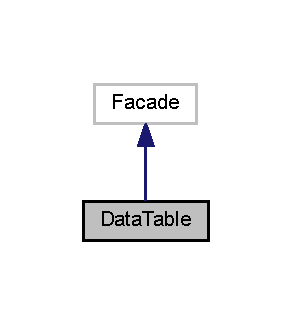
\includegraphics[width=140pt]{classhamburgscleanest_1_1_data_tables_1_1_facades_1_1_data_table__inherit__graph}
\end{center}
\end{figure}


Collaboration diagram for Data\+Table\+:
\nopagebreak
\begin{figure}[H]
\begin{center}
\leavevmode
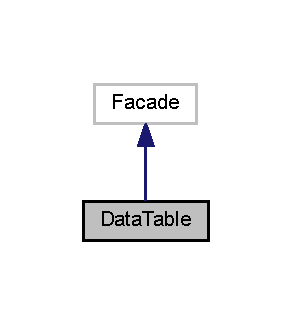
\includegraphics[width=140pt]{classhamburgscleanest_1_1_data_tables_1_1_facades_1_1_data_table__coll__graph}
\end{center}
\end{figure}
\subsection*{Static Protected Member Functions}
\begin{DoxyCompactItemize}
\item 
static \hyperlink{classhamburgscleanest_1_1_data_tables_1_1_facades_1_1_data_table_a19a808201f41f32f71a0532cb49b450f}{get\+Facade\+Accessor} ()
\end{DoxyCompactItemize}


\subsection{Member Function Documentation}
\mbox{\Hypertarget{classhamburgscleanest_1_1_data_tables_1_1_facades_1_1_data_table_a19a808201f41f32f71a0532cb49b450f}\label{classhamburgscleanest_1_1_data_tables_1_1_facades_1_1_data_table_a19a808201f41f32f71a0532cb49b450f}} 
\index{hamburgscleanest\+::\+Data\+Tables\+::\+Facades\+::\+Data\+Table@{hamburgscleanest\+::\+Data\+Tables\+::\+Facades\+::\+Data\+Table}!get\+Facade\+Accessor@{get\+Facade\+Accessor}}
\index{get\+Facade\+Accessor@{get\+Facade\+Accessor}!hamburgscleanest\+::\+Data\+Tables\+::\+Facades\+::\+Data\+Table@{hamburgscleanest\+::\+Data\+Tables\+::\+Facades\+::\+Data\+Table}}
\subsubsection{\texorpdfstring{get\+Facade\+Accessor()}{getFacadeAccessor()}}
{\footnotesize\ttfamily static get\+Facade\+Accessor (\begin{DoxyParamCaption}{ }\end{DoxyParamCaption})\hspace{0.3cm}{\ttfamily [static]}, {\ttfamily [protected]}}

Get the registered name of the component.

\begin{DoxyReturn}{Returns}
string 
\end{DoxyReturn}


The documentation for this class was generated from the following file\+:\begin{DoxyCompactItemize}
\item 
C\+:/\+Users/chrom/\+\_\+\+P\+A\+G\+E\+S/\+Package\+Dev/packages/hamburgscleanest/\+Data\+Tables/src/\+Facades/Data\+Table.\+php\end{DoxyCompactItemize}

\hypertarget{classhamburgscleanest_1_1_data_tables_1_1_data_tables_service_provider}{}\section{Data\+Tables\+Service\+Provider Class Reference}
\label{classhamburgscleanest_1_1_data_tables_1_1_data_tables_service_provider}\index{Data\+Tables\+Service\+Provider@{Data\+Tables\+Service\+Provider}}


Inheritance diagram for Data\+Tables\+Service\+Provider\+:
\nopagebreak
\begin{figure}[H]
\begin{center}
\leavevmode
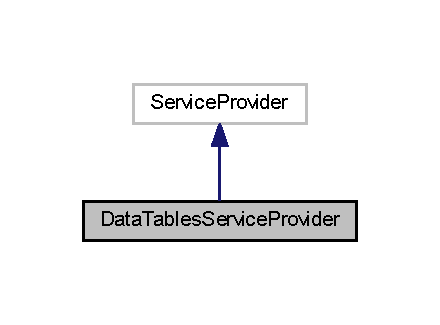
\includegraphics[width=211pt]{classhamburgscleanest_1_1_data_tables_1_1_data_tables_service_provider__inherit__graph}
\end{center}
\end{figure}


Collaboration diagram for Data\+Tables\+Service\+Provider\+:
\nopagebreak
\begin{figure}[H]
\begin{center}
\leavevmode
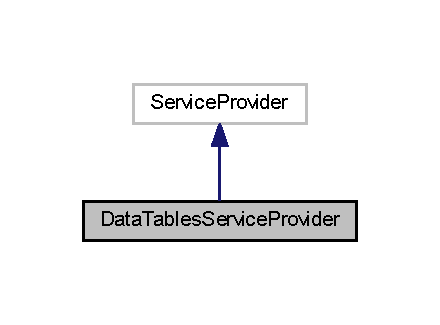
\includegraphics[width=211pt]{classhamburgscleanest_1_1_data_tables_1_1_data_tables_service_provider__coll__graph}
\end{center}
\end{figure}
\subsection*{Public Member Functions}
\begin{DoxyCompactItemize}
\item 
\hyperlink{classhamburgscleanest_1_1_data_tables_1_1_data_tables_service_provider_a8814ea4b5beba763c570b4818980814e}{boot} ()
\item 
\hyperlink{classhamburgscleanest_1_1_data_tables_1_1_data_tables_service_provider_acc294a6cc8e69743746820e3d15e3f78}{register} ()
\end{DoxyCompactItemize}


\subsection{Member Function Documentation}
\mbox{\Hypertarget{classhamburgscleanest_1_1_data_tables_1_1_data_tables_service_provider_a8814ea4b5beba763c570b4818980814e}\label{classhamburgscleanest_1_1_data_tables_1_1_data_tables_service_provider_a8814ea4b5beba763c570b4818980814e}} 
\index{hamburgscleanest\+::\+Data\+Tables\+::\+Data\+Tables\+Service\+Provider@{hamburgscleanest\+::\+Data\+Tables\+::\+Data\+Tables\+Service\+Provider}!boot@{boot}}
\index{boot@{boot}!hamburgscleanest\+::\+Data\+Tables\+::\+Data\+Tables\+Service\+Provider@{hamburgscleanest\+::\+Data\+Tables\+::\+Data\+Tables\+Service\+Provider}}
\subsubsection{\texorpdfstring{boot()}{boot()}}
{\footnotesize\ttfamily boot (\begin{DoxyParamCaption}{ }\end{DoxyParamCaption})}

Perform post-\/registration booting of services.

\begin{DoxyReturn}{Returns}
void 
\end{DoxyReturn}
\mbox{\Hypertarget{classhamburgscleanest_1_1_data_tables_1_1_data_tables_service_provider_acc294a6cc8e69743746820e3d15e3f78}\label{classhamburgscleanest_1_1_data_tables_1_1_data_tables_service_provider_acc294a6cc8e69743746820e3d15e3f78}} 
\index{hamburgscleanest\+::\+Data\+Tables\+::\+Data\+Tables\+Service\+Provider@{hamburgscleanest\+::\+Data\+Tables\+::\+Data\+Tables\+Service\+Provider}!register@{register}}
\index{register@{register}!hamburgscleanest\+::\+Data\+Tables\+::\+Data\+Tables\+Service\+Provider@{hamburgscleanest\+::\+Data\+Tables\+::\+Data\+Tables\+Service\+Provider}}
\subsubsection{\texorpdfstring{register()}{register()}}
{\footnotesize\ttfamily register (\begin{DoxyParamCaption}{ }\end{DoxyParamCaption})}

Register any package services.

\begin{DoxyReturn}{Returns}
void 
\end{DoxyReturn}


The documentation for this class was generated from the following file\+:\begin{DoxyCompactItemize}
\item 
C\+:/\+Users/chrom/\+\_\+\+P\+A\+G\+E\+S/\+Package\+Dev/packages/hamburgscleanest/\+Data\+Tables/src/Data\+Tables\+Service\+Provider.\+php\end{DoxyCompactItemize}

\hypertarget{classhamburgscleanest_1_1_data_tables_1_1_models_1_1_column_formatters_1_1_date_column}{}\section{Date\+Column Class Reference}
\label{classhamburgscleanest_1_1_data_tables_1_1_models_1_1_column_formatters_1_1_date_column}\index{Date\+Column@{Date\+Column}}


Inheritance diagram for Date\+Column\+:
\nopagebreak
\begin{figure}[H]
\begin{center}
\leavevmode
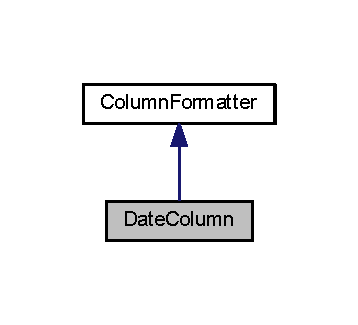
\includegraphics[width=172pt]{classhamburgscleanest_1_1_data_tables_1_1_models_1_1_column_formatters_1_1_date_column__inherit__graph}
\end{center}
\end{figure}


Collaboration diagram for Date\+Column\+:
\nopagebreak
\begin{figure}[H]
\begin{center}
\leavevmode
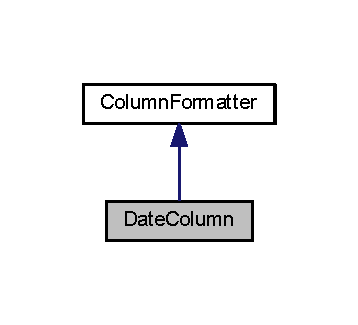
\includegraphics[width=172pt]{classhamburgscleanest_1_1_data_tables_1_1_models_1_1_column_formatters_1_1_date_column__coll__graph}
\end{center}
\end{figure}
\subsection*{Public Member Functions}
\begin{DoxyCompactItemize}
\item 
\hyperlink{classhamburgscleanest_1_1_data_tables_1_1_models_1_1_column_formatters_1_1_date_column_a0115f0c68a42cda38a3ab35261da68ec}{\+\_\+\+\_\+construct} (string \$\hyperlink{classhamburgscleanest_1_1_data_tables_1_1_models_1_1_column_formatters_1_1_date_column_a6ab68973747a78d533feb978aaf8eebc}{date\+Format}=\textquotesingle{}Y-\/m-\/d H\+:i\+:s\textquotesingle{})
\item 
\hyperlink{classhamburgscleanest_1_1_data_tables_1_1_models_1_1_column_formatters_1_1_date_column_a6ab68973747a78d533feb978aaf8eebc}{date\+Format} (string \$date\+Format)
\item 
\hyperlink{classhamburgscleanest_1_1_data_tables_1_1_models_1_1_column_formatters_1_1_date_column_aba259f7ae8b25e70bd444020c04606e7}{format} (string \$column)
\end{DoxyCompactItemize}


\subsection{Constructor \& Destructor Documentation}
\mbox{\Hypertarget{classhamburgscleanest_1_1_data_tables_1_1_models_1_1_column_formatters_1_1_date_column_a0115f0c68a42cda38a3ab35261da68ec}\label{classhamburgscleanest_1_1_data_tables_1_1_models_1_1_column_formatters_1_1_date_column_a0115f0c68a42cda38a3ab35261da68ec}} 
\index{hamburgscleanest\+::\+Data\+Tables\+::\+Models\+::\+Column\+Formatters\+::\+Date\+Column@{hamburgscleanest\+::\+Data\+Tables\+::\+Models\+::\+Column\+Formatters\+::\+Date\+Column}!\+\_\+\+\_\+construct@{\+\_\+\+\_\+construct}}
\index{\+\_\+\+\_\+construct@{\+\_\+\+\_\+construct}!hamburgscleanest\+::\+Data\+Tables\+::\+Models\+::\+Column\+Formatters\+::\+Date\+Column@{hamburgscleanest\+::\+Data\+Tables\+::\+Models\+::\+Column\+Formatters\+::\+Date\+Column}}
\subsubsection{\texorpdfstring{\+\_\+\+\_\+construct()}{\_\_construct()}}
{\footnotesize\ttfamily \+\_\+\+\_\+construct (\begin{DoxyParamCaption}\item[{string}]{\$date\+Format = {\ttfamily \textquotesingle{}Y-\/m-\/d~H\+:i\+:s\textquotesingle{}} }\end{DoxyParamCaption})}

\hyperlink{classhamburgscleanest_1_1_data_tables_1_1_models_1_1_column_formatters_1_1_date_column}{Date\+Column} constructor. 
\begin{DoxyParams}[1]{Parameters}
string & {\em \$date\+Format} & \\
\hline
\end{DoxyParams}


\subsection{Member Function Documentation}
\mbox{\Hypertarget{classhamburgscleanest_1_1_data_tables_1_1_models_1_1_column_formatters_1_1_date_column_a6ab68973747a78d533feb978aaf8eebc}\label{classhamburgscleanest_1_1_data_tables_1_1_models_1_1_column_formatters_1_1_date_column_a6ab68973747a78d533feb978aaf8eebc}} 
\index{hamburgscleanest\+::\+Data\+Tables\+::\+Models\+::\+Column\+Formatters\+::\+Date\+Column@{hamburgscleanest\+::\+Data\+Tables\+::\+Models\+::\+Column\+Formatters\+::\+Date\+Column}!date\+Format@{date\+Format}}
\index{date\+Format@{date\+Format}!hamburgscleanest\+::\+Data\+Tables\+::\+Models\+::\+Column\+Formatters\+::\+Date\+Column@{hamburgscleanest\+::\+Data\+Tables\+::\+Models\+::\+Column\+Formatters\+::\+Date\+Column}}
\subsubsection{\texorpdfstring{date\+Format()}{dateFormat()}}
{\footnotesize\ttfamily date\+Format (\begin{DoxyParamCaption}\item[{string}]{\$date\+Format }\end{DoxyParamCaption})}

Set the format of the date column, e.\+g. \char`\"{}\+Y-\/m-\/d H\+:i\+:s\char`\"{}.


\begin{DoxyParams}[1]{Parameters}
string & {\em \$date\+Format} & \\
\hline
\end{DoxyParams}
\begin{DoxyReturn}{Returns}
\hyperlink{classhamburgscleanest_1_1_data_tables_1_1_models_1_1_column_formatters_1_1_date_column}{Date\+Column} 
\end{DoxyReturn}
\mbox{\Hypertarget{classhamburgscleanest_1_1_data_tables_1_1_models_1_1_column_formatters_1_1_date_column_aba259f7ae8b25e70bd444020c04606e7}\label{classhamburgscleanest_1_1_data_tables_1_1_models_1_1_column_formatters_1_1_date_column_aba259f7ae8b25e70bd444020c04606e7}} 
\index{hamburgscleanest\+::\+Data\+Tables\+::\+Models\+::\+Column\+Formatters\+::\+Date\+Column@{hamburgscleanest\+::\+Data\+Tables\+::\+Models\+::\+Column\+Formatters\+::\+Date\+Column}!format@{format}}
\index{format@{format}!hamburgscleanest\+::\+Data\+Tables\+::\+Models\+::\+Column\+Formatters\+::\+Date\+Column@{hamburgscleanest\+::\+Data\+Tables\+::\+Models\+::\+Column\+Formatters\+::\+Date\+Column}}
\subsubsection{\texorpdfstring{format()}{format()}}
{\footnotesize\ttfamily format (\begin{DoxyParamCaption}\item[{string}]{\$column }\end{DoxyParamCaption})}


\begin{DoxyParams}[1]{Parameters}
string & {\em \$column} & \\
\hline
\end{DoxyParams}
\begin{DoxyReturn}{Returns}
string 
\end{DoxyReturn}


Implements \hyperlink{interfacehamburgscleanest_1_1_data_tables_1_1_interfaces_1_1_column_formatter_aba259f7ae8b25e70bd444020c04606e7}{Column\+Formatter}.



The documentation for this class was generated from the following file\+:\begin{DoxyCompactItemize}
\item 
C\+:/\+Users/chrom/\+\_\+\+P\+A\+G\+E\+S/\+Package\+Dev/packages/hamburgscleanest/\+Data\+Tables/src/\+Models/\+Column\+Formatters/Date\+Column.\+php\end{DoxyCompactItemize}

\hypertarget{classhamburgscleanest_1_1_data_tables_1_1_models_1_1_header}{}\section{Header Class Reference}
\label{classhamburgscleanest_1_1_data_tables_1_1_models_1_1_header}\index{Header@{Header}}
\subsection*{Public Member Functions}
\begin{DoxyCompactItemize}
\item 
\hyperlink{classhamburgscleanest_1_1_data_tables_1_1_models_1_1_header_ab9936a9a68205e1e45d06b26f1563221}{\+\_\+\+\_\+construct} (string \$column\+Key)
\item 
\hyperlink{classhamburgscleanest_1_1_data_tables_1_1_models_1_1_header_aef428fd06c26df985591f168f4387ddf}{get\+Attribute\+Name} ()
\item 
\hyperlink{classhamburgscleanest_1_1_data_tables_1_1_models_1_1_header_adbfe1566856df6d9c2570c9941a39db6}{format\+Array} (array \$header\+Formatters)
\item 
\hyperlink{classhamburgscleanest_1_1_data_tables_1_1_models_1_1_header_a3d535bcef2cd83c8f69efd922b8ac939}{format} (\hyperlink{interfacehamburgscleanest_1_1_data_tables_1_1_interfaces_1_1_header_formatter}{Header\+Formatter} \$header\+Formatter)
\item 
\hyperlink{classhamburgscleanest_1_1_data_tables_1_1_models_1_1_header_a43374e600f552e0a9308ab96b1964aba}{print} ()
\end{DoxyCompactItemize}
\subsection*{Data Fields}
\begin{DoxyCompactItemize}
\item 
\mbox{\Hypertarget{classhamburgscleanest_1_1_data_tables_1_1_models_1_1_header_aa60b0284e0dfa2463495481cf11e3cf4}\label{classhamburgscleanest_1_1_data_tables_1_1_models_1_1_header_aa60b0284e0dfa2463495481cf11e3cf4}} 
{\bfseries \$key}
\end{DoxyCompactItemize}


\subsection{Constructor \& Destructor Documentation}
\mbox{\Hypertarget{classhamburgscleanest_1_1_data_tables_1_1_models_1_1_header_ab9936a9a68205e1e45d06b26f1563221}\label{classhamburgscleanest_1_1_data_tables_1_1_models_1_1_header_ab9936a9a68205e1e45d06b26f1563221}} 
\index{hamburgscleanest\+::\+Data\+Tables\+::\+Models\+::\+Header@{hamburgscleanest\+::\+Data\+Tables\+::\+Models\+::\+Header}!\+\_\+\+\_\+construct@{\+\_\+\+\_\+construct}}
\index{\+\_\+\+\_\+construct@{\+\_\+\+\_\+construct}!hamburgscleanest\+::\+Data\+Tables\+::\+Models\+::\+Header@{hamburgscleanest\+::\+Data\+Tables\+::\+Models\+::\+Header}}
\subsubsection{\texorpdfstring{\+\_\+\+\_\+construct()}{\_\_construct()}}
{\footnotesize\ttfamily \+\_\+\+\_\+construct (\begin{DoxyParamCaption}\item[{string}]{\$column\+Key }\end{DoxyParamCaption})}

\hyperlink{classhamburgscleanest_1_1_data_tables_1_1_models_1_1_header}{Header} constructor. 
\begin{DoxyParams}[1]{Parameters}
string & {\em \$column\+Key} & \\
\hline
\end{DoxyParams}


\subsection{Member Function Documentation}
\mbox{\Hypertarget{classhamburgscleanest_1_1_data_tables_1_1_models_1_1_header_a3d535bcef2cd83c8f69efd922b8ac939}\label{classhamburgscleanest_1_1_data_tables_1_1_models_1_1_header_a3d535bcef2cd83c8f69efd922b8ac939}} 
\index{hamburgscleanest\+::\+Data\+Tables\+::\+Models\+::\+Header@{hamburgscleanest\+::\+Data\+Tables\+::\+Models\+::\+Header}!format@{format}}
\index{format@{format}!hamburgscleanest\+::\+Data\+Tables\+::\+Models\+::\+Header@{hamburgscleanest\+::\+Data\+Tables\+::\+Models\+::\+Header}}
\subsubsection{\texorpdfstring{format()}{format()}}
{\footnotesize\ttfamily format (\begin{DoxyParamCaption}\item[{\hyperlink{interfacehamburgscleanest_1_1_data_tables_1_1_interfaces_1_1_header_formatter}{Header\+Formatter}}]{\$header\+Formatter }\end{DoxyParamCaption})}


\begin{DoxyParams}[1]{Parameters}
Header\+Formatter & {\em \$header\+Formatter} & \\
\hline
\end{DoxyParams}
\begin{DoxyReturn}{Returns}
\hyperlink{classhamburgscleanest_1_1_data_tables_1_1_models_1_1_header}{Header} 
\end{DoxyReturn}
\mbox{\Hypertarget{classhamburgscleanest_1_1_data_tables_1_1_models_1_1_header_adbfe1566856df6d9c2570c9941a39db6}\label{classhamburgscleanest_1_1_data_tables_1_1_models_1_1_header_adbfe1566856df6d9c2570c9941a39db6}} 
\index{hamburgscleanest\+::\+Data\+Tables\+::\+Models\+::\+Header@{hamburgscleanest\+::\+Data\+Tables\+::\+Models\+::\+Header}!format\+Array@{format\+Array}}
\index{format\+Array@{format\+Array}!hamburgscleanest\+::\+Data\+Tables\+::\+Models\+::\+Header@{hamburgscleanest\+::\+Data\+Tables\+::\+Models\+::\+Header}}
\subsubsection{\texorpdfstring{format\+Array()}{formatArray()}}
{\footnotesize\ttfamily format\+Array (\begin{DoxyParamCaption}\item[{array}]{\$header\+Formatters }\end{DoxyParamCaption})}


\begin{DoxyParams}[1]{Parameters}
array & {\em \$header\+Formatters} & \\
\hline
\end{DoxyParams}
\begin{DoxyReturn}{Returns}
\hyperlink{classhamburgscleanest_1_1_data_tables_1_1_models_1_1_header}{Header} 
\end{DoxyReturn}
\mbox{\Hypertarget{classhamburgscleanest_1_1_data_tables_1_1_models_1_1_header_aef428fd06c26df985591f168f4387ddf}\label{classhamburgscleanest_1_1_data_tables_1_1_models_1_1_header_aef428fd06c26df985591f168f4387ddf}} 
\index{hamburgscleanest\+::\+Data\+Tables\+::\+Models\+::\+Header@{hamburgscleanest\+::\+Data\+Tables\+::\+Models\+::\+Header}!get\+Attribute\+Name@{get\+Attribute\+Name}}
\index{get\+Attribute\+Name@{get\+Attribute\+Name}!hamburgscleanest\+::\+Data\+Tables\+::\+Models\+::\+Header@{hamburgscleanest\+::\+Data\+Tables\+::\+Models\+::\+Header}}
\subsubsection{\texorpdfstring{get\+Attribute\+Name()}{getAttributeName()}}
{\footnotesize\ttfamily get\+Attribute\+Name (\begin{DoxyParamCaption}{ }\end{DoxyParamCaption})}

Get the original attribute name.

\begin{DoxyReturn}{Returns}
string 
\end{DoxyReturn}
\mbox{\Hypertarget{classhamburgscleanest_1_1_data_tables_1_1_models_1_1_header_a43374e600f552e0a9308ab96b1964aba}\label{classhamburgscleanest_1_1_data_tables_1_1_models_1_1_header_a43374e600f552e0a9308ab96b1964aba}} 
\index{hamburgscleanest\+::\+Data\+Tables\+::\+Models\+::\+Header@{hamburgscleanest\+::\+Data\+Tables\+::\+Models\+::\+Header}!print@{print}}
\index{print@{print}!hamburgscleanest\+::\+Data\+Tables\+::\+Models\+::\+Header@{hamburgscleanest\+::\+Data\+Tables\+::\+Models\+::\+Header}}
\subsubsection{\texorpdfstring{print()}{print()}}
{\footnotesize\ttfamily print (\begin{DoxyParamCaption}{ }\end{DoxyParamCaption})}

\begin{DoxyReturn}{Returns}
string 
\end{DoxyReturn}


The documentation for this class was generated from the following file\+:\begin{DoxyCompactItemize}
\item 
C\+:/\+Users/chrom/\+\_\+\+P\+A\+G\+E\+S/\+Package\+Dev/packages/hamburgscleanest/\+Data\+Tables/src/\+Models/Header.\+php\end{DoxyCompactItemize}

\hypertarget{interfacehamburgscleanest_1_1_data_tables_1_1_interfaces_1_1_header_formatter}{}\section{Header\+Formatter Interface Reference}
\label{interfacehamburgscleanest_1_1_data_tables_1_1_interfaces_1_1_header_formatter}\index{Header\+Formatter@{Header\+Formatter}}


Inheritance diagram for Header\+Formatter\+:\nopagebreak
\begin{figure}[H]
\begin{center}
\leavevmode
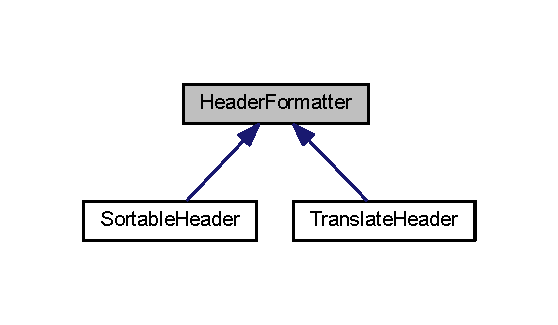
\includegraphics[width=268pt]{interfacehamburgscleanest_1_1_data_tables_1_1_interfaces_1_1_header_formatter__inherit__graph}
\end{center}
\end{figure}
\subsection*{Public Member Functions}
\begin{DoxyCompactItemize}
\item 
\hyperlink{interfacehamburgscleanest_1_1_data_tables_1_1_interfaces_1_1_header_formatter_aa5aeddf9c056d9583b29322f75f70f82}{format} (\hyperlink{classhamburgscleanest_1_1_data_tables_1_1_models_1_1_header}{Header} \$header)
\end{DoxyCompactItemize}


\subsection{Member Function Documentation}
\mbox{\Hypertarget{interfacehamburgscleanest_1_1_data_tables_1_1_interfaces_1_1_header_formatter_aa5aeddf9c056d9583b29322f75f70f82}\label{interfacehamburgscleanest_1_1_data_tables_1_1_interfaces_1_1_header_formatter_aa5aeddf9c056d9583b29322f75f70f82}} 
\index{hamburgscleanest\+::\+Data\+Tables\+::\+Interfaces\+::\+Header\+Formatter@{hamburgscleanest\+::\+Data\+Tables\+::\+Interfaces\+::\+Header\+Formatter}!format@{format}}
\index{format@{format}!hamburgscleanest\+::\+Data\+Tables\+::\+Interfaces\+::\+Header\+Formatter@{hamburgscleanest\+::\+Data\+Tables\+::\+Interfaces\+::\+Header\+Formatter}}
\subsubsection{\texorpdfstring{format()}{format()}}
{\footnotesize\ttfamily format (\begin{DoxyParamCaption}\item[{\hyperlink{classhamburgscleanest_1_1_data_tables_1_1_models_1_1_header}{Header}}]{\$header }\end{DoxyParamCaption})}

Format the given header. For example add a link to sort by this header/column.


\begin{DoxyParams}[1]{Parameters}
Header & {\em \$header} & \\
\hline
\end{DoxyParams}
\begin{DoxyReturn}{Returns}
void 
\end{DoxyReturn}


Implemented in \hyperlink{classhamburgscleanest_1_1_data_tables_1_1_models_1_1_header_formatters_1_1_sortable_header_aa5aeddf9c056d9583b29322f75f70f82}{Sortable\+Header}, and \hyperlink{classhamburgscleanest_1_1_data_tables_1_1_models_1_1_header_formatters_1_1_translate_header_aa5aeddf9c056d9583b29322f75f70f82}{Translate\+Header}.



The documentation for this interface was generated from the following file\+:\begin{DoxyCompactItemize}
\item 
C\+:/\+Users/chrom/\+\_\+\+P\+A\+G\+E\+S/\+Package\+Dev/packages/hamburgscleanest/\+Data\+Tables/src/\+Interfaces/Header\+Formatter.\+php\end{DoxyCompactItemize}

\hypertarget{classhamburgscleanest_1_1_data_tables_1_1_models_1_1_data_components_1_1_paginator}{}\section{Paginator Class Reference}
\label{classhamburgscleanest_1_1_data_tables_1_1_models_1_1_data_components_1_1_paginator}\index{Paginator@{Paginator}}


Inheritance diagram for Paginator\+:\nopagebreak
\begin{figure}[H]
\begin{center}
\leavevmode
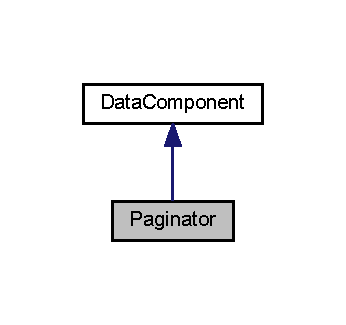
\includegraphics[width=166pt]{classhamburgscleanest_1_1_data_tables_1_1_models_1_1_data_components_1_1_paginator__inherit__graph}
\end{center}
\end{figure}


Collaboration diagram for Paginator\+:\nopagebreak
\begin{figure}[H]
\begin{center}
\leavevmode
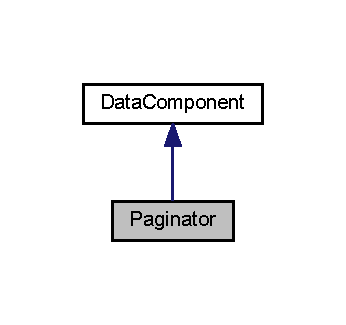
\includegraphics[width=166pt]{classhamburgscleanest_1_1_data_tables_1_1_models_1_1_data_components_1_1_paginator__coll__graph}
\end{center}
\end{figure}
\subsection*{Public Member Functions}
\begin{DoxyCompactItemize}
\item 
\hyperlink{classhamburgscleanest_1_1_data_tables_1_1_models_1_1_data_components_1_1_paginator_abc3963927c17e1a03f685cafe82e217b}{\+\_\+\+\_\+construct} (int \$per\+Page=15)
\item 
\hyperlink{classhamburgscleanest_1_1_data_tables_1_1_models_1_1_data_components_1_1_paginator_a5e68817e5b1382d72237b5b0aa0c543e}{entries\+Per\+Page} (\$per\+Page=15)
\item 
\hyperlink{classhamburgscleanest_1_1_data_tables_1_1_models_1_1_data_components_1_1_paginator_ab4a99d48dee7f0f1202d66439dbc0c5b}{surrounding\+Pages} (\$count=2)
\item 
\hyperlink{classhamburgscleanest_1_1_data_tables_1_1_models_1_1_data_components_1_1_paginator_afde88292c44dc59faf017738dae6dffb}{render} ()
\item 
\hyperlink{classhamburgscleanest_1_1_data_tables_1_1_models_1_1_data_components_1_1_paginator_a29cca2e4eba71144e202922486e55e99}{page\+Count} ()
\end{DoxyCompactItemize}
\subsection*{Protected Member Functions}
\begin{DoxyCompactItemize}
\item 
\hyperlink{classhamburgscleanest_1_1_data_tables_1_1_models_1_1_data_components_1_1_paginator_a6d4fda1024fd883f0750e5f0c531160d}{\+\_\+shape\+Data} ()
\item 
\mbox{\Hypertarget{classhamburgscleanest_1_1_data_tables_1_1_models_1_1_data_components_1_1_paginator_a8b97dff3fa609aaed04b448e535ba0cc}\label{classhamburgscleanest_1_1_data_tables_1_1_models_1_1_data_components_1_1_paginator_a8b97dff3fa609aaed04b448e535ba0cc}} 
{\bfseries \+\_\+after\+Init} ()
\end{DoxyCompactItemize}
\subsection*{Additional Inherited Members}


\subsection{Constructor \& Destructor Documentation}
\mbox{\Hypertarget{classhamburgscleanest_1_1_data_tables_1_1_models_1_1_data_components_1_1_paginator_abc3963927c17e1a03f685cafe82e217b}\label{classhamburgscleanest_1_1_data_tables_1_1_models_1_1_data_components_1_1_paginator_abc3963927c17e1a03f685cafe82e217b}} 
\index{hamburgscleanest\+::\+Data\+Tables\+::\+Models\+::\+Data\+Components\+::\+Paginator@{hamburgscleanest\+::\+Data\+Tables\+::\+Models\+::\+Data\+Components\+::\+Paginator}!\+\_\+\+\_\+construct@{\+\_\+\+\_\+construct}}
\index{\+\_\+\+\_\+construct@{\+\_\+\+\_\+construct}!hamburgscleanest\+::\+Data\+Tables\+::\+Models\+::\+Data\+Components\+::\+Paginator@{hamburgscleanest\+::\+Data\+Tables\+::\+Models\+::\+Data\+Components\+::\+Paginator}}
\subsubsection{\texorpdfstring{\+\_\+\+\_\+construct()}{\_\_construct()}}
{\footnotesize\ttfamily \+\_\+\+\_\+construct (\begin{DoxyParamCaption}\item[{int}]{\$per\+Page = {\ttfamily 15} }\end{DoxyParamCaption})}

\hyperlink{classhamburgscleanest_1_1_data_tables_1_1_models_1_1_data_components_1_1_paginator}{Paginator} constructor. 
\begin{DoxyParams}[1]{Parameters}
int & {\em \$per\+Page} & \\
\hline
\end{DoxyParams}


\subsection{Member Function Documentation}
\mbox{\Hypertarget{classhamburgscleanest_1_1_data_tables_1_1_models_1_1_data_components_1_1_paginator_a6d4fda1024fd883f0750e5f0c531160d}\label{classhamburgscleanest_1_1_data_tables_1_1_models_1_1_data_components_1_1_paginator_a6d4fda1024fd883f0750e5f0c531160d}} 
\index{hamburgscleanest\+::\+Data\+Tables\+::\+Models\+::\+Data\+Components\+::\+Paginator@{hamburgscleanest\+::\+Data\+Tables\+::\+Models\+::\+Data\+Components\+::\+Paginator}!\+\_\+shape\+Data@{\+\_\+shape\+Data}}
\index{\+\_\+shape\+Data@{\+\_\+shape\+Data}!hamburgscleanest\+::\+Data\+Tables\+::\+Models\+::\+Data\+Components\+::\+Paginator@{hamburgscleanest\+::\+Data\+Tables\+::\+Models\+::\+Data\+Components\+::\+Paginator}}
\subsubsection{\texorpdfstring{\+\_\+shape\+Data()}{\_shapeData()}}
{\footnotesize\ttfamily \+\_\+shape\+Data (\begin{DoxyParamCaption}{ }\end{DoxyParamCaption})\hspace{0.3cm}{\ttfamily [protected]}}

\begin{DoxyReturn}{Returns}
Builder 
\end{DoxyReturn}
\mbox{\Hypertarget{classhamburgscleanest_1_1_data_tables_1_1_models_1_1_data_components_1_1_paginator_a5e68817e5b1382d72237b5b0aa0c543e}\label{classhamburgscleanest_1_1_data_tables_1_1_models_1_1_data_components_1_1_paginator_a5e68817e5b1382d72237b5b0aa0c543e}} 
\index{hamburgscleanest\+::\+Data\+Tables\+::\+Models\+::\+Data\+Components\+::\+Paginator@{hamburgscleanest\+::\+Data\+Tables\+::\+Models\+::\+Data\+Components\+::\+Paginator}!entries\+Per\+Page@{entries\+Per\+Page}}
\index{entries\+Per\+Page@{entries\+Per\+Page}!hamburgscleanest\+::\+Data\+Tables\+::\+Models\+::\+Data\+Components\+::\+Paginator@{hamburgscleanest\+::\+Data\+Tables\+::\+Models\+::\+Data\+Components\+::\+Paginator}}
\subsubsection{\texorpdfstring{entries\+Per\+Page()}{entriesPerPage()}}
{\footnotesize\ttfamily entries\+Per\+Page (\begin{DoxyParamCaption}\item[{}]{\$per\+Page = {\ttfamily 15} }\end{DoxyParamCaption})}

How many entries per page?


\begin{DoxyParams}[1]{Parameters}
int & {\em \$per\+Page} & \\
\hline
\end{DoxyParams}
\begin{DoxyReturn}{Returns}
\hyperlink{classhamburgscleanest_1_1_data_tables_1_1_models_1_1_data_components_1_1_paginator}{Paginator} 
\end{DoxyReturn}
\mbox{\Hypertarget{classhamburgscleanest_1_1_data_tables_1_1_models_1_1_data_components_1_1_paginator_a29cca2e4eba71144e202922486e55e99}\label{classhamburgscleanest_1_1_data_tables_1_1_models_1_1_data_components_1_1_paginator_a29cca2e4eba71144e202922486e55e99}} 
\index{hamburgscleanest\+::\+Data\+Tables\+::\+Models\+::\+Data\+Components\+::\+Paginator@{hamburgscleanest\+::\+Data\+Tables\+::\+Models\+::\+Data\+Components\+::\+Paginator}!page\+Count@{page\+Count}}
\index{page\+Count@{page\+Count}!hamburgscleanest\+::\+Data\+Tables\+::\+Models\+::\+Data\+Components\+::\+Paginator@{hamburgscleanest\+::\+Data\+Tables\+::\+Models\+::\+Data\+Components\+::\+Paginator}}
\subsubsection{\texorpdfstring{page\+Count()}{pageCount()}}
{\footnotesize\ttfamily page\+Count (\begin{DoxyParamCaption}{ }\end{DoxyParamCaption})}

\begin{DoxyReturn}{Returns}
int 
\end{DoxyReturn}
\mbox{\Hypertarget{classhamburgscleanest_1_1_data_tables_1_1_models_1_1_data_components_1_1_paginator_afde88292c44dc59faf017738dae6dffb}\label{classhamburgscleanest_1_1_data_tables_1_1_models_1_1_data_components_1_1_paginator_afde88292c44dc59faf017738dae6dffb}} 
\index{hamburgscleanest\+::\+Data\+Tables\+::\+Models\+::\+Data\+Components\+::\+Paginator@{hamburgscleanest\+::\+Data\+Tables\+::\+Models\+::\+Data\+Components\+::\+Paginator}!render@{render}}
\index{render@{render}!hamburgscleanest\+::\+Data\+Tables\+::\+Models\+::\+Data\+Components\+::\+Paginator@{hamburgscleanest\+::\+Data\+Tables\+::\+Models\+::\+Data\+Components\+::\+Paginator}}
\subsubsection{\texorpdfstring{render()}{render()}}
{\footnotesize\ttfamily render (\begin{DoxyParamCaption}{ }\end{DoxyParamCaption})}

Render the page links.

\begin{DoxyReturn}{Returns}
string 
\end{DoxyReturn}

\begin{DoxyExceptions}{Exceptions}
{\em } & \\
\hline
\end{DoxyExceptions}
\mbox{\Hypertarget{classhamburgscleanest_1_1_data_tables_1_1_models_1_1_data_components_1_1_paginator_ab4a99d48dee7f0f1202d66439dbc0c5b}\label{classhamburgscleanest_1_1_data_tables_1_1_models_1_1_data_components_1_1_paginator_ab4a99d48dee7f0f1202d66439dbc0c5b}} 
\index{hamburgscleanest\+::\+Data\+Tables\+::\+Models\+::\+Data\+Components\+::\+Paginator@{hamburgscleanest\+::\+Data\+Tables\+::\+Models\+::\+Data\+Components\+::\+Paginator}!surrounding\+Pages@{surrounding\+Pages}}
\index{surrounding\+Pages@{surrounding\+Pages}!hamburgscleanest\+::\+Data\+Tables\+::\+Models\+::\+Data\+Components\+::\+Paginator@{hamburgscleanest\+::\+Data\+Tables\+::\+Models\+::\+Data\+Components\+::\+Paginator}}
\subsubsection{\texorpdfstring{surrounding\+Pages()}{surroundingPages()}}
{\footnotesize\ttfamily surrounding\+Pages (\begin{DoxyParamCaption}\item[{}]{\$count = {\ttfamily 2} }\end{DoxyParamCaption})}

How many surrounding pages should be shown?


\begin{DoxyParams}[1]{Parameters}
int & {\em \$count} & \\
\hline
\end{DoxyParams}
\begin{DoxyReturn}{Returns}
\hyperlink{classhamburgscleanest_1_1_data_tables_1_1_models_1_1_data_components_1_1_paginator}{Paginator} 
\end{DoxyReturn}


The documentation for this class was generated from the following file\+:\begin{DoxyCompactItemize}
\item 
C\+:/\+Users/chrom/\+\_\+\+P\+A\+G\+E\+S/\+Package\+Dev/packages/hamburgscleanest/\+Data\+Tables/src/\+Models/\+Data\+Components/Paginator.\+php\end{DoxyCompactItemize}

\hypertarget{classhamburgscleanest_1_1_data_tables_1_1_models_1_1_relation}{}\section{Relation Class Reference}
\label{classhamburgscleanest_1_1_data_tables_1_1_models_1_1_relation}\index{Relation@{Relation}}
\subsection*{Public Member Functions}
\begin{DoxyCompactItemize}
\item 
\hyperlink{classhamburgscleanest_1_1_data_tables_1_1_models_1_1_relation_a32982fa61bdbcb31c04986b55a015422}{\+\_\+\+\_\+construct} (string \$column\+Name)
\item 
\hyperlink{classhamburgscleanest_1_1_data_tables_1_1_models_1_1_relation_a2706c7287269d1fe90002ec71b629c80}{get\+Value} (string \$column\+Name, Collection \$relation)
\end{DoxyCompactItemize}
\subsection*{Data Fields}
\begin{DoxyCompactItemize}
\item 
\mbox{\Hypertarget{classhamburgscleanest_1_1_data_tables_1_1_models_1_1_relation_ab2fc40d43824ea3e1ce5d86dee0d763b}\label{classhamburgscleanest_1_1_data_tables_1_1_models_1_1_relation_ab2fc40d43824ea3e1ce5d86dee0d763b}} 
{\bfseries \$name}
\item 
\mbox{\Hypertarget{classhamburgscleanest_1_1_data_tables_1_1_models_1_1_relation_a64886274e81c8152b822038ab683dbe1}\label{classhamburgscleanest_1_1_data_tables_1_1_models_1_1_relation_a64886274e81c8152b822038ab683dbe1}} 
{\bfseries \$aggregate} = \textquotesingle{}first\textquotesingle{}
\item 
\mbox{\Hypertarget{classhamburgscleanest_1_1_data_tables_1_1_models_1_1_relation_a257bb27c360747a7f80b842e7109f54c}\label{classhamburgscleanest_1_1_data_tables_1_1_models_1_1_relation_a257bb27c360747a7f80b842e7109f54c}} 
{\bfseries \$attribute\+Name}
\end{DoxyCompactItemize}


\subsection{Constructor \& Destructor Documentation}
\mbox{\Hypertarget{classhamburgscleanest_1_1_data_tables_1_1_models_1_1_relation_a32982fa61bdbcb31c04986b55a015422}\label{classhamburgscleanest_1_1_data_tables_1_1_models_1_1_relation_a32982fa61bdbcb31c04986b55a015422}} 
\index{hamburgscleanest\+::\+Data\+Tables\+::\+Models\+::\+Relation@{hamburgscleanest\+::\+Data\+Tables\+::\+Models\+::\+Relation}!\+\_\+\+\_\+construct@{\+\_\+\+\_\+construct}}
\index{\+\_\+\+\_\+construct@{\+\_\+\+\_\+construct}!hamburgscleanest\+::\+Data\+Tables\+::\+Models\+::\+Relation@{hamburgscleanest\+::\+Data\+Tables\+::\+Models\+::\+Relation}}
\subsubsection{\texorpdfstring{\+\_\+\+\_\+construct()}{\_\_construct()}}
{\footnotesize\ttfamily \+\_\+\+\_\+construct (\begin{DoxyParamCaption}\item[{string}]{\$column\+Name }\end{DoxyParamCaption})}

\hyperlink{classhamburgscleanest_1_1_data_tables_1_1_models_1_1_relation}{Relation} constructor. 
\begin{DoxyParams}[1]{Parameters}
string & {\em \$column\+Name} & \\
\hline
\end{DoxyParams}


\subsection{Member Function Documentation}
\mbox{\Hypertarget{classhamburgscleanest_1_1_data_tables_1_1_models_1_1_relation_a2706c7287269d1fe90002ec71b629c80}\label{classhamburgscleanest_1_1_data_tables_1_1_models_1_1_relation_a2706c7287269d1fe90002ec71b629c80}} 
\index{hamburgscleanest\+::\+Data\+Tables\+::\+Models\+::\+Relation@{hamburgscleanest\+::\+Data\+Tables\+::\+Models\+::\+Relation}!get\+Value@{get\+Value}}
\index{get\+Value@{get\+Value}!hamburgscleanest\+::\+Data\+Tables\+::\+Models\+::\+Relation@{hamburgscleanest\+::\+Data\+Tables\+::\+Models\+::\+Relation}}
\subsubsection{\texorpdfstring{get\+Value()}{getValue()}}
{\footnotesize\ttfamily get\+Value (\begin{DoxyParamCaption}\item[{string}]{\$column\+Name,  }\item[{Collection}]{\$relation }\end{DoxyParamCaption})}


\begin{DoxyParams}[1]{Parameters}
string & {\em \$column\+Name} & \\
\hline
Collection & {\em \$relation} & \\
\hline
\end{DoxyParams}
\begin{DoxyReturn}{Returns}
string 
\end{DoxyReturn}


The documentation for this class was generated from the following file\+:\begin{DoxyCompactItemize}
\item 
C\+:/\+Users/chrom/\+\_\+\+P\+A\+G\+E\+S/\+Package\+Dev/packages/hamburgscleanest/\+Data\+Tables/src/\+Models/Relation.\+php\end{DoxyCompactItemize}

\hypertarget{classhamburgscleanest_1_1_data_tables_1_1_facades_1_1_session_helper}{}\section{Session\+Helper Class Reference}
\label{classhamburgscleanest_1_1_data_tables_1_1_facades_1_1_session_helper}\index{Session\+Helper@{Session\+Helper}}


Inheritance diagram for Session\+Helper\+:\nopagebreak
\begin{figure}[H]
\begin{center}
\leavevmode
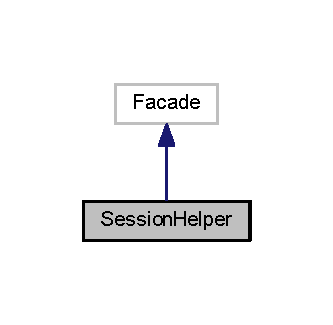
\includegraphics[width=160pt]{classhamburgscleanest_1_1_data_tables_1_1_facades_1_1_session_helper__inherit__graph}
\end{center}
\end{figure}


Collaboration diagram for Session\+Helper\+:\nopagebreak
\begin{figure}[H]
\begin{center}
\leavevmode
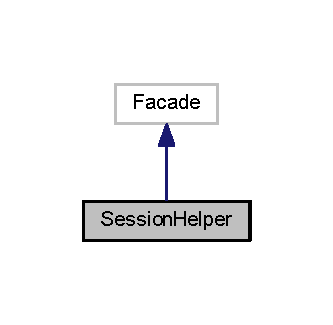
\includegraphics[width=160pt]{classhamburgscleanest_1_1_data_tables_1_1_facades_1_1_session_helper__coll__graph}
\end{center}
\end{figure}
\subsection*{Static Protected Member Functions}
\begin{DoxyCompactItemize}
\item 
static \hyperlink{classhamburgscleanest_1_1_data_tables_1_1_facades_1_1_session_helper_a19a808201f41f32f71a0532cb49b450f}{get\+Facade\+Accessor} ()
\end{DoxyCompactItemize}


\subsection{Member Function Documentation}
\mbox{\Hypertarget{classhamburgscleanest_1_1_data_tables_1_1_facades_1_1_session_helper_a19a808201f41f32f71a0532cb49b450f}\label{classhamburgscleanest_1_1_data_tables_1_1_facades_1_1_session_helper_a19a808201f41f32f71a0532cb49b450f}} 
\index{hamburgscleanest\+::\+Data\+Tables\+::\+Facades\+::\+Session\+Helper@{hamburgscleanest\+::\+Data\+Tables\+::\+Facades\+::\+Session\+Helper}!get\+Facade\+Accessor@{get\+Facade\+Accessor}}
\index{get\+Facade\+Accessor@{get\+Facade\+Accessor}!hamburgscleanest\+::\+Data\+Tables\+::\+Facades\+::\+Session\+Helper@{hamburgscleanest\+::\+Data\+Tables\+::\+Facades\+::\+Session\+Helper}}
\subsubsection{\texorpdfstring{get\+Facade\+Accessor()}{getFacadeAccessor()}}
{\footnotesize\ttfamily static get\+Facade\+Accessor (\begin{DoxyParamCaption}{ }\end{DoxyParamCaption})\hspace{0.3cm}{\ttfamily [static]}, {\ttfamily [protected]}}

Get the registered name of the component.

\begin{DoxyReturn}{Returns}
string 
\end{DoxyReturn}


The documentation for this class was generated from the following file\+:\begin{DoxyCompactItemize}
\item 
C\+:/\+Users/chrom/\+\_\+\+P\+A\+G\+E\+S/\+Package\+Dev/packages/hamburgscleanest/\+Data\+Tables/src/\+Facades/Session\+Helper.\+php\end{DoxyCompactItemize}

\hypertarget{classhamburgscleanest_1_1_data_tables_1_1_helpers_1_1_session_helper}{}\section{Session\+Helper Class Reference}
\label{classhamburgscleanest_1_1_data_tables_1_1_helpers_1_1_session_helper}\index{Session\+Helper@{Session\+Helper}}
\subsection*{Public Member Functions}
\begin{DoxyCompactItemize}
\item 
\hyperlink{classhamburgscleanest_1_1_data_tables_1_1_helpers_1_1_session_helper_a2b2f57e8efe838cbb1a61ffc3e1f1aa6}{save\+State} (string \$key, \$session\+Value)
\item 
\hyperlink{classhamburgscleanest_1_1_data_tables_1_1_helpers_1_1_session_helper_a213f24f847d58eb033424decc2039c62}{get\+State} (string \$key, \$default=null)
\item 
\hyperlink{classhamburgscleanest_1_1_data_tables_1_1_helpers_1_1_session_helper_a1672adb7d32dc37bdaeb0bd1ff92a0f7}{remove\+State} (string \$key)
\end{DoxyCompactItemize}
\subsection*{Data Fields}
\begin{DoxyCompactItemize}
\item 
\mbox{\Hypertarget{classhamburgscleanest_1_1_data_tables_1_1_helpers_1_1_session_helper_a3f80c5b5eade75883410c851751a1420}\label{classhamburgscleanest_1_1_data_tables_1_1_helpers_1_1_session_helper_a3f80c5b5eade75883410c851751a1420}} 
const {\bfseries S\+E\+S\+S\+I\+O\+N\+\_\+\+S\+T\+O\+R\+A\+GE} = \textquotesingle{}data-\/tables.\textquotesingle{}
\end{DoxyCompactItemize}


\subsection{Member Function Documentation}
\mbox{\Hypertarget{classhamburgscleanest_1_1_data_tables_1_1_helpers_1_1_session_helper_a213f24f847d58eb033424decc2039c62}\label{classhamburgscleanest_1_1_data_tables_1_1_helpers_1_1_session_helper_a213f24f847d58eb033424decc2039c62}} 
\index{hamburgscleanest\+::\+Data\+Tables\+::\+Helpers\+::\+Session\+Helper@{hamburgscleanest\+::\+Data\+Tables\+::\+Helpers\+::\+Session\+Helper}!get\+State@{get\+State}}
\index{get\+State@{get\+State}!hamburgscleanest\+::\+Data\+Tables\+::\+Helpers\+::\+Session\+Helper@{hamburgscleanest\+::\+Data\+Tables\+::\+Helpers\+::\+Session\+Helper}}
\subsubsection{\texorpdfstring{get\+State()}{getState()}}
{\footnotesize\ttfamily get\+State (\begin{DoxyParamCaption}\item[{string}]{\$key,  }\item[{}]{\$default = {\ttfamily null} }\end{DoxyParamCaption})}

Get the state for the given key.


\begin{DoxyParams}[1]{Parameters}
string & {\em \$key} & \\
\hline
null & {\em \$default} & \\
\hline
\end{DoxyParams}
\begin{DoxyReturn}{Returns}
mixed 
\end{DoxyReturn}

\begin{DoxyExceptions}{Exceptions}
{\em } & \\
\hline
\end{DoxyExceptions}
\mbox{\Hypertarget{classhamburgscleanest_1_1_data_tables_1_1_helpers_1_1_session_helper_a1672adb7d32dc37bdaeb0bd1ff92a0f7}\label{classhamburgscleanest_1_1_data_tables_1_1_helpers_1_1_session_helper_a1672adb7d32dc37bdaeb0bd1ff92a0f7}} 
\index{hamburgscleanest\+::\+Data\+Tables\+::\+Helpers\+::\+Session\+Helper@{hamburgscleanest\+::\+Data\+Tables\+::\+Helpers\+::\+Session\+Helper}!remove\+State@{remove\+State}}
\index{remove\+State@{remove\+State}!hamburgscleanest\+::\+Data\+Tables\+::\+Helpers\+::\+Session\+Helper@{hamburgscleanest\+::\+Data\+Tables\+::\+Helpers\+::\+Session\+Helper}}
\subsubsection{\texorpdfstring{remove\+State()}{removeState()}}
{\footnotesize\ttfamily remove\+State (\begin{DoxyParamCaption}\item[{string}]{\$key }\end{DoxyParamCaption})}

Remove the state for the given key.


\begin{DoxyParams}[1]{Parameters}
string & {\em \$key} & \\
\hline
\end{DoxyParams}

\begin{DoxyExceptions}{Exceptions}
{\em } & \\
\hline
\end{DoxyExceptions}
\mbox{\Hypertarget{classhamburgscleanest_1_1_data_tables_1_1_helpers_1_1_session_helper_a2b2f57e8efe838cbb1a61ffc3e1f1aa6}\label{classhamburgscleanest_1_1_data_tables_1_1_helpers_1_1_session_helper_a2b2f57e8efe838cbb1a61ffc3e1f1aa6}} 
\index{hamburgscleanest\+::\+Data\+Tables\+::\+Helpers\+::\+Session\+Helper@{hamburgscleanest\+::\+Data\+Tables\+::\+Helpers\+::\+Session\+Helper}!save\+State@{save\+State}}
\index{save\+State@{save\+State}!hamburgscleanest\+::\+Data\+Tables\+::\+Helpers\+::\+Session\+Helper@{hamburgscleanest\+::\+Data\+Tables\+::\+Helpers\+::\+Session\+Helper}}
\subsubsection{\texorpdfstring{save\+State()}{saveState()}}
{\footnotesize\ttfamily save\+State (\begin{DoxyParamCaption}\item[{string}]{\$key,  }\item[{}]{\$session\+Value }\end{DoxyParamCaption})}

Save the state for the given key.


\begin{DoxyParams}[1]{Parameters}
string & {\em \$key} & \\
\hline
mixed & {\em \$session\+Value} & \\
\hline
\end{DoxyParams}

\begin{DoxyExceptions}{Exceptions}
{\em } & \\
\hline
\end{DoxyExceptions}


The documentation for this class was generated from the following file\+:\begin{DoxyCompactItemize}
\item 
C\+:/\+Users/chrom/\+\_\+\+P\+A\+G\+E\+S/\+Package\+Dev/packages/hamburgscleanest/\+Data\+Tables/src/\+Helpers/Session\+Helper.\+php\end{DoxyCompactItemize}

\hypertarget{classhamburgscleanest_1_1_data_tables_1_1_models_1_1_header_formatters_1_1_sortable_header}{}\section{Sortable\+Header Class Reference}
\label{classhamburgscleanest_1_1_data_tables_1_1_models_1_1_header_formatters_1_1_sortable_header}\index{Sortable\+Header@{Sortable\+Header}}


Inheritance diagram for Sortable\+Header\+:
\nopagebreak
\begin{figure}[H]
\begin{center}
\leavevmode
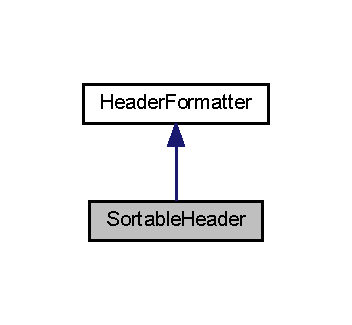
\includegraphics[width=169pt]{classhamburgscleanest_1_1_data_tables_1_1_models_1_1_header_formatters_1_1_sortable_header__inherit__graph}
\end{center}
\end{figure}


Collaboration diagram for Sortable\+Header\+:
\nopagebreak
\begin{figure}[H]
\begin{center}
\leavevmode
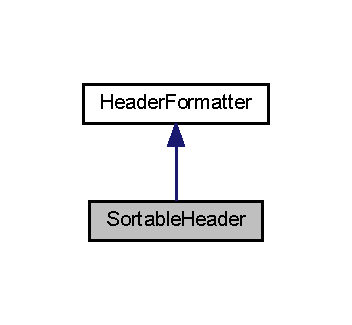
\includegraphics[width=169pt]{classhamburgscleanest_1_1_data_tables_1_1_models_1_1_header_formatters_1_1_sortable_header__coll__graph}
\end{center}
\end{figure}
\subsection*{Public Member Functions}
\begin{DoxyCompactItemize}
\item 
\hyperlink{classhamburgscleanest_1_1_data_tables_1_1_models_1_1_header_formatters_1_1_sortable_header_ae425990a4233288ed86fc75dc6059738}{\+\_\+\+\_\+construct} (array \$sortable\+Headers=\mbox{[}$\,$\mbox{]}, array \$\hyperlink{classhamburgscleanest_1_1_data_tables_1_1_models_1_1_header_formatters_1_1_sortable_header_afac8d813b0a89bf0c7c6ce1c7a053dfd}{dont\+Sort}=\mbox{[}$\,$\mbox{]})
\item 
\hyperlink{classhamburgscleanest_1_1_data_tables_1_1_models_1_1_header_formatters_1_1_sortable_header_a85a83d247ad5c4e8c00fe00b646b031c}{sorting\+Symbols} (array \$sorting\+Symbols)
\item 
\hyperlink{classhamburgscleanest_1_1_data_tables_1_1_models_1_1_header_formatters_1_1_sortable_header_ac59bec60dbfa5e8cf5009736b4d07068}{make\+Sortable} (string \$header)
\item 
\hyperlink{classhamburgscleanest_1_1_data_tables_1_1_models_1_1_header_formatters_1_1_sortable_header_afac8d813b0a89bf0c7c6ce1c7a053dfd}{dont\+Sort} (string \$header)
\item 
\hyperlink{classhamburgscleanest_1_1_data_tables_1_1_models_1_1_header_formatters_1_1_sortable_header_aa5aeddf9c056d9583b29322f75f70f82}{format} (\hyperlink{classhamburgscleanest_1_1_data_tables_1_1_models_1_1_header}{Header} \$header)
\end{DoxyCompactItemize}
\subsection*{Data Fields}
\begin{DoxyCompactItemize}
\item 
\mbox{\Hypertarget{classhamburgscleanest_1_1_data_tables_1_1_models_1_1_header_formatters_1_1_sortable_header_a087c53f1298172fcd6792a9e6d094786}\label{classhamburgscleanest_1_1_data_tables_1_1_models_1_1_header_formatters_1_1_sortable_header_a087c53f1298172fcd6792a9e6d094786}} 
const {\bfseries S\+O\+R\+T\+I\+N\+G\+\_\+\+S\+E\+P\+A\+R\+A\+T\+OR} = \textquotesingle{}$\sim$\textquotesingle{}
\item 
\mbox{\Hypertarget{classhamburgscleanest_1_1_data_tables_1_1_models_1_1_header_formatters_1_1_sortable_header_a3506ba6f9fa4c5bb1fa04da91367e6bd}\label{classhamburgscleanest_1_1_data_tables_1_1_models_1_1_header_formatters_1_1_sortable_header_a3506ba6f9fa4c5bb1fa04da91367e6bd}} 
const {\bfseries C\+O\+L\+U\+M\+N\+\_\+\+S\+E\+P\+A\+R\+A\+T\+OR} = \textquotesingle{}.\textquotesingle{}
\end{DoxyCompactItemize}


\subsection{Constructor \& Destructor Documentation}
\mbox{\Hypertarget{classhamburgscleanest_1_1_data_tables_1_1_models_1_1_header_formatters_1_1_sortable_header_ae425990a4233288ed86fc75dc6059738}\label{classhamburgscleanest_1_1_data_tables_1_1_models_1_1_header_formatters_1_1_sortable_header_ae425990a4233288ed86fc75dc6059738}} 
\index{hamburgscleanest\+::\+Data\+Tables\+::\+Models\+::\+Header\+Formatters\+::\+Sortable\+Header@{hamburgscleanest\+::\+Data\+Tables\+::\+Models\+::\+Header\+Formatters\+::\+Sortable\+Header}!\+\_\+\+\_\+construct@{\+\_\+\+\_\+construct}}
\index{\+\_\+\+\_\+construct@{\+\_\+\+\_\+construct}!hamburgscleanest\+::\+Data\+Tables\+::\+Models\+::\+Header\+Formatters\+::\+Sortable\+Header@{hamburgscleanest\+::\+Data\+Tables\+::\+Models\+::\+Header\+Formatters\+::\+Sortable\+Header}}
\subsubsection{\texorpdfstring{\+\_\+\+\_\+construct()}{\_\_construct()}}
{\footnotesize\ttfamily \+\_\+\+\_\+construct (\begin{DoxyParamCaption}\item[{array}]{\$sortable\+Headers = {\ttfamily \mbox{[}\mbox{]}},  }\item[{array}]{\$dont\+Sort = {\ttfamily \mbox{[}\mbox{]}} }\end{DoxyParamCaption})}

\hyperlink{classhamburgscleanest_1_1_data_tables_1_1_models_1_1_header_formatters_1_1_sortable_header}{Sortable\+Header} constructor.


\begin{DoxyParams}[1]{Parameters}
array & {\em \$sortable\+Headers} & \\
\hline
array & {\em \$dont\+Sort} & \\
\hline
\end{DoxyParams}


\subsection{Member Function Documentation}
\mbox{\Hypertarget{classhamburgscleanest_1_1_data_tables_1_1_models_1_1_header_formatters_1_1_sortable_header_afac8d813b0a89bf0c7c6ce1c7a053dfd}\label{classhamburgscleanest_1_1_data_tables_1_1_models_1_1_header_formatters_1_1_sortable_header_afac8d813b0a89bf0c7c6ce1c7a053dfd}} 
\index{hamburgscleanest\+::\+Data\+Tables\+::\+Models\+::\+Header\+Formatters\+::\+Sortable\+Header@{hamburgscleanest\+::\+Data\+Tables\+::\+Models\+::\+Header\+Formatters\+::\+Sortable\+Header}!dont\+Sort@{dont\+Sort}}
\index{dont\+Sort@{dont\+Sort}!hamburgscleanest\+::\+Data\+Tables\+::\+Models\+::\+Header\+Formatters\+::\+Sortable\+Header@{hamburgscleanest\+::\+Data\+Tables\+::\+Models\+::\+Header\+Formatters\+::\+Sortable\+Header}}
\subsubsection{\texorpdfstring{dont\+Sort()}{dontSort()}}
{\footnotesize\ttfamily dont\+Sort (\begin{DoxyParamCaption}\item[{string}]{\$header }\end{DoxyParamCaption})}

Remove the ability to sort by this column/header.


\begin{DoxyParams}[1]{Parameters}
string & {\em \$header} & \\
\hline
\end{DoxyParams}
\begin{DoxyReturn}{Returns}
\hyperlink{classhamburgscleanest_1_1_data_tables_1_1_models_1_1_header_formatters_1_1_sortable_header}{Sortable\+Header} 
\end{DoxyReturn}
\mbox{\Hypertarget{classhamburgscleanest_1_1_data_tables_1_1_models_1_1_header_formatters_1_1_sortable_header_aa5aeddf9c056d9583b29322f75f70f82}\label{classhamburgscleanest_1_1_data_tables_1_1_models_1_1_header_formatters_1_1_sortable_header_aa5aeddf9c056d9583b29322f75f70f82}} 
\index{hamburgscleanest\+::\+Data\+Tables\+::\+Models\+::\+Header\+Formatters\+::\+Sortable\+Header@{hamburgscleanest\+::\+Data\+Tables\+::\+Models\+::\+Header\+Formatters\+::\+Sortable\+Header}!format@{format}}
\index{format@{format}!hamburgscleanest\+::\+Data\+Tables\+::\+Models\+::\+Header\+Formatters\+::\+Sortable\+Header@{hamburgscleanest\+::\+Data\+Tables\+::\+Models\+::\+Header\+Formatters\+::\+Sortable\+Header}}
\subsubsection{\texorpdfstring{format()}{format()}}
{\footnotesize\ttfamily format (\begin{DoxyParamCaption}\item[{\hyperlink{classhamburgscleanest_1_1_data_tables_1_1_models_1_1_header}{Header}}]{\$header }\end{DoxyParamCaption})}

Adds a link to sort by this header/column. Also indicates how the columns are sorted (when sorted).


\begin{DoxyParams}[1]{Parameters}
\hyperlink{classhamburgscleanest_1_1_data_tables_1_1_models_1_1_header}{Header} & {\em \$header} & \\
\hline
\end{DoxyParams}

\begin{DoxyExceptions}{Exceptions}
{\em } & \\
\hline
\end{DoxyExceptions}


Implements \hyperlink{interfacehamburgscleanest_1_1_data_tables_1_1_interfaces_1_1_header_formatter_aa5aeddf9c056d9583b29322f75f70f82}{Header\+Formatter}.

\mbox{\Hypertarget{classhamburgscleanest_1_1_data_tables_1_1_models_1_1_header_formatters_1_1_sortable_header_ac59bec60dbfa5e8cf5009736b4d07068}\label{classhamburgscleanest_1_1_data_tables_1_1_models_1_1_header_formatters_1_1_sortable_header_ac59bec60dbfa5e8cf5009736b4d07068}} 
\index{hamburgscleanest\+::\+Data\+Tables\+::\+Models\+::\+Header\+Formatters\+::\+Sortable\+Header@{hamburgscleanest\+::\+Data\+Tables\+::\+Models\+::\+Header\+Formatters\+::\+Sortable\+Header}!make\+Sortable@{make\+Sortable}}
\index{make\+Sortable@{make\+Sortable}!hamburgscleanest\+::\+Data\+Tables\+::\+Models\+::\+Header\+Formatters\+::\+Sortable\+Header@{hamburgscleanest\+::\+Data\+Tables\+::\+Models\+::\+Header\+Formatters\+::\+Sortable\+Header}}
\subsubsection{\texorpdfstring{make\+Sortable()}{makeSortable()}}
{\footnotesize\ttfamily make\+Sortable (\begin{DoxyParamCaption}\item[{string}]{\$header }\end{DoxyParamCaption})}

Add a field to the sortable fields.


\begin{DoxyParams}[1]{Parameters}
string & {\em \$header} & \\
\hline
\end{DoxyParams}
\begin{DoxyReturn}{Returns}
\hyperlink{classhamburgscleanest_1_1_data_tables_1_1_models_1_1_header_formatters_1_1_sortable_header}{Sortable\+Header} 
\end{DoxyReturn}
\mbox{\Hypertarget{classhamburgscleanest_1_1_data_tables_1_1_models_1_1_header_formatters_1_1_sortable_header_a85a83d247ad5c4e8c00fe00b646b031c}\label{classhamburgscleanest_1_1_data_tables_1_1_models_1_1_header_formatters_1_1_sortable_header_a85a83d247ad5c4e8c00fe00b646b031c}} 
\index{hamburgscleanest\+::\+Data\+Tables\+::\+Models\+::\+Header\+Formatters\+::\+Sortable\+Header@{hamburgscleanest\+::\+Data\+Tables\+::\+Models\+::\+Header\+Formatters\+::\+Sortable\+Header}!sorting\+Symbols@{sorting\+Symbols}}
\index{sorting\+Symbols@{sorting\+Symbols}!hamburgscleanest\+::\+Data\+Tables\+::\+Models\+::\+Header\+Formatters\+::\+Sortable\+Header@{hamburgscleanest\+::\+Data\+Tables\+::\+Models\+::\+Header\+Formatters\+::\+Sortable\+Header}}
\subsubsection{\texorpdfstring{sorting\+Symbols()}{sortingSymbols()}}
{\footnotesize\ttfamily sorting\+Symbols (\begin{DoxyParamCaption}\item[{array}]{\$sorting\+Symbols }\end{DoxyParamCaption})}


\begin{DoxyParams}[1]{Parameters}
array & {\em \$sorting\+Symbols} & \\
\hline
\end{DoxyParams}
\begin{DoxyReturn}{Returns}
\hyperlink{classhamburgscleanest_1_1_data_tables_1_1_models_1_1_header_formatters_1_1_sortable_header}{Sortable\+Header} 
\end{DoxyReturn}


The documentation for this class was generated from the following file\+:\begin{DoxyCompactItemize}
\item 
C\+:/\+Users/chrom/\+\_\+\+P\+A\+G\+E\+S/\+Package\+Dev/packages/hamburgscleanest/\+Data\+Tables/src/\+Models/\+Header\+Formatters/Sortable\+Header.\+php\end{DoxyCompactItemize}

\hypertarget{classhamburgscleanest_1_1_data_tables_1_1_models_1_1_data_components_1_1_sorter}{}\section{Sorter Class Reference}
\label{classhamburgscleanest_1_1_data_tables_1_1_models_1_1_data_components_1_1_sorter}\index{Sorter@{Sorter}}


Inheritance diagram for Sorter\+:\nopagebreak
\begin{figure}[H]
\begin{center}
\leavevmode
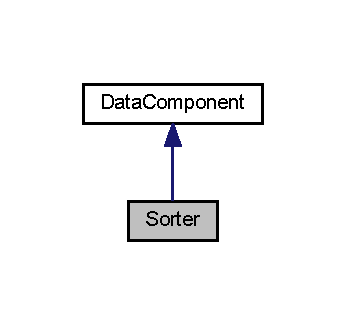
\includegraphics[width=166pt]{classhamburgscleanest_1_1_data_tables_1_1_models_1_1_data_components_1_1_sorter__inherit__graph}
\end{center}
\end{figure}


Collaboration diagram for Sorter\+:\nopagebreak
\begin{figure}[H]
\begin{center}
\leavevmode
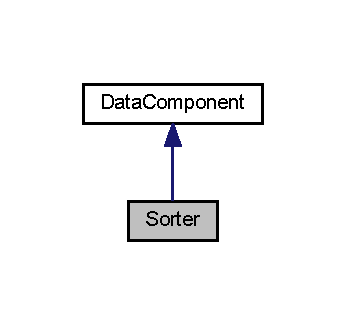
\includegraphics[width=166pt]{classhamburgscleanest_1_1_data_tables_1_1_models_1_1_data_components_1_1_sorter__coll__graph}
\end{center}
\end{figure}
\subsection*{Public Member Functions}
\begin{DoxyCompactItemize}
\item 
\hyperlink{classhamburgscleanest_1_1_data_tables_1_1_models_1_1_data_components_1_1_sorter_a0d814929f87d0f11eeadf759faf05fcb}{\+\_\+\+\_\+construct} (array \$fields=null, bool \$\hyperlink{classhamburgscleanest_1_1_data_tables_1_1_models_1_1_data_component_a565ac6563f3548952f5b3b9807799d17}{remember}=false)
\item 
\hyperlink{classhamburgscleanest_1_1_data_tables_1_1_models_1_1_data_components_1_1_sorter_aa5b9b656f19ab3777d6a2ad013c648fc}{add\+Field} (string \$field, string \$direction=\textquotesingle{}asc\textquotesingle{})
\item 
\hyperlink{classhamburgscleanest_1_1_data_tables_1_1_models_1_1_data_components_1_1_sorter_afde88292c44dc59faf017738dae6dffb}{render} ()
\item 
\hyperlink{classhamburgscleanest_1_1_data_tables_1_1_models_1_1_data_components_1_1_sorter_aa4c3f30fa02501d5020e400bef11a9bb}{remove\+Field} (string \$field)
\end{DoxyCompactItemize}
\subsection*{Data Fields}
\begin{DoxyCompactItemize}
\item 
\mbox{\Hypertarget{classhamburgscleanest_1_1_data_tables_1_1_models_1_1_data_components_1_1_sorter_a087c53f1298172fcd6792a9e6d094786}\label{classhamburgscleanest_1_1_data_tables_1_1_models_1_1_data_components_1_1_sorter_a087c53f1298172fcd6792a9e6d094786}} 
const {\bfseries S\+O\+R\+T\+I\+N\+G\+\_\+\+S\+E\+P\+A\+R\+A\+T\+OR} = \textquotesingle{}$\sim$\textquotesingle{}
\item 
\mbox{\Hypertarget{classhamburgscleanest_1_1_data_tables_1_1_models_1_1_data_components_1_1_sorter_a3506ba6f9fa4c5bb1fa04da91367e6bd}\label{classhamburgscleanest_1_1_data_tables_1_1_models_1_1_data_components_1_1_sorter_a3506ba6f9fa4c5bb1fa04da91367e6bd}} 
const {\bfseries C\+O\+L\+U\+M\+N\+\_\+\+S\+E\+P\+A\+R\+A\+T\+OR} = \textquotesingle{}.\textquotesingle{}
\end{DoxyCompactItemize}
\subsection*{Protected Member Functions}
\begin{DoxyCompactItemize}
\item 
\hyperlink{classhamburgscleanest_1_1_data_tables_1_1_models_1_1_data_components_1_1_sorter_a6d4fda1024fd883f0750e5f0c531160d}{\+\_\+shape\+Data} ()
\item 
\mbox{\Hypertarget{classhamburgscleanest_1_1_data_tables_1_1_models_1_1_data_components_1_1_sorter_ae682ac7f1f1f9516c3cc2485ae5bcf4b}\label{classhamburgscleanest_1_1_data_tables_1_1_models_1_1_data_components_1_1_sorter_ae682ac7f1f1f9516c3cc2485ae5bcf4b}} 
{\bfseries \+\_\+read\+From\+Session} ()
\item 
\mbox{\Hypertarget{classhamburgscleanest_1_1_data_tables_1_1_models_1_1_data_components_1_1_sorter_a28881ca4bf07d4008e3ed3128198da59}\label{classhamburgscleanest_1_1_data_tables_1_1_models_1_1_data_components_1_1_sorter_a28881ca4bf07d4008e3ed3128198da59}} 
{\bfseries \+\_\+store\+In\+Session} ()
\end{DoxyCompactItemize}
\subsection*{Additional Inherited Members}


\subsection{Constructor \& Destructor Documentation}
\mbox{\Hypertarget{classhamburgscleanest_1_1_data_tables_1_1_models_1_1_data_components_1_1_sorter_a0d814929f87d0f11eeadf759faf05fcb}\label{classhamburgscleanest_1_1_data_tables_1_1_models_1_1_data_components_1_1_sorter_a0d814929f87d0f11eeadf759faf05fcb}} 
\index{hamburgscleanest\+::\+Data\+Tables\+::\+Models\+::\+Data\+Components\+::\+Sorter@{hamburgscleanest\+::\+Data\+Tables\+::\+Models\+::\+Data\+Components\+::\+Sorter}!\+\_\+\+\_\+construct@{\+\_\+\+\_\+construct}}
\index{\+\_\+\+\_\+construct@{\+\_\+\+\_\+construct}!hamburgscleanest\+::\+Data\+Tables\+::\+Models\+::\+Data\+Components\+::\+Sorter@{hamburgscleanest\+::\+Data\+Tables\+::\+Models\+::\+Data\+Components\+::\+Sorter}}
\subsubsection{\texorpdfstring{\+\_\+\+\_\+construct()}{\_\_construct()}}
{\footnotesize\ttfamily \+\_\+\+\_\+construct (\begin{DoxyParamCaption}\item[{array}]{\$fields = {\ttfamily null},  }\item[{bool}]{\$remember = {\ttfamily false} }\end{DoxyParamCaption})}

\hyperlink{classhamburgscleanest_1_1_data_tables_1_1_models_1_1_data_components_1_1_sorter}{Sorter} constructor. 
\begin{DoxyParams}[1]{Parameters}
null | array & {\em \$fields} & \\
\hline
bool & {\em \$remember} & \\
\hline
\end{DoxyParams}


\subsection{Member Function Documentation}
\mbox{\Hypertarget{classhamburgscleanest_1_1_data_tables_1_1_models_1_1_data_components_1_1_sorter_a6d4fda1024fd883f0750e5f0c531160d}\label{classhamburgscleanest_1_1_data_tables_1_1_models_1_1_data_components_1_1_sorter_a6d4fda1024fd883f0750e5f0c531160d}} 
\index{hamburgscleanest\+::\+Data\+Tables\+::\+Models\+::\+Data\+Components\+::\+Sorter@{hamburgscleanest\+::\+Data\+Tables\+::\+Models\+::\+Data\+Components\+::\+Sorter}!\+\_\+shape\+Data@{\+\_\+shape\+Data}}
\index{\+\_\+shape\+Data@{\+\_\+shape\+Data}!hamburgscleanest\+::\+Data\+Tables\+::\+Models\+::\+Data\+Components\+::\+Sorter@{hamburgscleanest\+::\+Data\+Tables\+::\+Models\+::\+Data\+Components\+::\+Sorter}}
\subsubsection{\texorpdfstring{\+\_\+shape\+Data()}{\_shapeData()}}
{\footnotesize\ttfamily \+\_\+shape\+Data (\begin{DoxyParamCaption}{ }\end{DoxyParamCaption})\hspace{0.3cm}{\ttfamily [protected]}}

\begin{DoxyReturn}{Returns}
Builder 
\end{DoxyReturn}
\mbox{\Hypertarget{classhamburgscleanest_1_1_data_tables_1_1_models_1_1_data_components_1_1_sorter_aa5b9b656f19ab3777d6a2ad013c648fc}\label{classhamburgscleanest_1_1_data_tables_1_1_models_1_1_data_components_1_1_sorter_aa5b9b656f19ab3777d6a2ad013c648fc}} 
\index{hamburgscleanest\+::\+Data\+Tables\+::\+Models\+::\+Data\+Components\+::\+Sorter@{hamburgscleanest\+::\+Data\+Tables\+::\+Models\+::\+Data\+Components\+::\+Sorter}!add\+Field@{add\+Field}}
\index{add\+Field@{add\+Field}!hamburgscleanest\+::\+Data\+Tables\+::\+Models\+::\+Data\+Components\+::\+Sorter@{hamburgscleanest\+::\+Data\+Tables\+::\+Models\+::\+Data\+Components\+::\+Sorter}}
\subsubsection{\texorpdfstring{add\+Field()}{addField()}}
{\footnotesize\ttfamily add\+Field (\begin{DoxyParamCaption}\item[{string}]{\$field,  }\item[{string}]{\$direction = {\ttfamily \textquotesingle{}asc\textquotesingle{}} }\end{DoxyParamCaption})}

Sort by this column.


\begin{DoxyParams}[1]{Parameters}
string & {\em \$field} & \\
\hline
string & {\em \$direction} & \\
\hline
\end{DoxyParams}
\begin{DoxyReturn}{Returns}
\hyperlink{classhamburgscleanest_1_1_data_tables_1_1_models_1_1_data_components_1_1_sorter}{Sorter} 
\end{DoxyReturn}
\mbox{\Hypertarget{classhamburgscleanest_1_1_data_tables_1_1_models_1_1_data_components_1_1_sorter_aa4c3f30fa02501d5020e400bef11a9bb}\label{classhamburgscleanest_1_1_data_tables_1_1_models_1_1_data_components_1_1_sorter_aa4c3f30fa02501d5020e400bef11a9bb}} 
\index{hamburgscleanest\+::\+Data\+Tables\+::\+Models\+::\+Data\+Components\+::\+Sorter@{hamburgscleanest\+::\+Data\+Tables\+::\+Models\+::\+Data\+Components\+::\+Sorter}!remove\+Field@{remove\+Field}}
\index{remove\+Field@{remove\+Field}!hamburgscleanest\+::\+Data\+Tables\+::\+Models\+::\+Data\+Components\+::\+Sorter@{hamburgscleanest\+::\+Data\+Tables\+::\+Models\+::\+Data\+Components\+::\+Sorter}}
\subsubsection{\texorpdfstring{remove\+Field()}{removeField()}}
{\footnotesize\ttfamily remove\+Field (\begin{DoxyParamCaption}\item[{string}]{\$field }\end{DoxyParamCaption})}

Stop sorting by this column


\begin{DoxyParams}[1]{Parameters}
string & {\em \$field} & \\
\hline
\end{DoxyParams}
\begin{DoxyReturn}{Returns}
\hyperlink{classhamburgscleanest_1_1_data_tables_1_1_models_1_1_data_components_1_1_sorter}{Sorter} 
\end{DoxyReturn}
\mbox{\Hypertarget{classhamburgscleanest_1_1_data_tables_1_1_models_1_1_data_components_1_1_sorter_afde88292c44dc59faf017738dae6dffb}\label{classhamburgscleanest_1_1_data_tables_1_1_models_1_1_data_components_1_1_sorter_afde88292c44dc59faf017738dae6dffb}} 
\index{hamburgscleanest\+::\+Data\+Tables\+::\+Models\+::\+Data\+Components\+::\+Sorter@{hamburgscleanest\+::\+Data\+Tables\+::\+Models\+::\+Data\+Components\+::\+Sorter}!render@{render}}
\index{render@{render}!hamburgscleanest\+::\+Data\+Tables\+::\+Models\+::\+Data\+Components\+::\+Sorter@{hamburgscleanest\+::\+Data\+Tables\+::\+Models\+::\+Data\+Components\+::\+Sorter}}
\subsubsection{\texorpdfstring{render()}{render()}}
{\footnotesize\ttfamily render (\begin{DoxyParamCaption}{ }\end{DoxyParamCaption})}

\begin{DoxyReturn}{Returns}
string 
\end{DoxyReturn}


The documentation for this class was generated from the following file\+:\begin{DoxyCompactItemize}
\item 
C\+:/\+Users/chrom/\+\_\+\+P\+A\+G\+E\+S/\+Package\+Dev/packages/hamburgscleanest/\+Data\+Tables/src/\+Models/\+Data\+Components/Sorter.\+php\end{DoxyCompactItemize}

\hypertarget{classhamburgscleanest_1_1_data_tables_1_1_facades_1_1_table_renderer}{}\section{Table\+Renderer Class Reference}
\label{classhamburgscleanest_1_1_data_tables_1_1_facades_1_1_table_renderer}\index{Table\+Renderer@{Table\+Renderer}}


Inheritance diagram for Table\+Renderer\+:\nopagebreak
\begin{figure}[H]
\begin{center}
\leavevmode
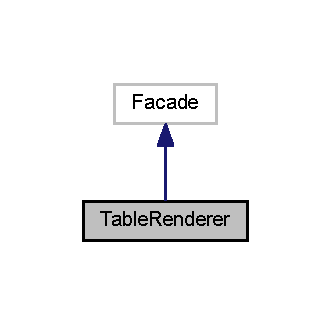
\includegraphics[width=159pt]{classhamburgscleanest_1_1_data_tables_1_1_facades_1_1_table_renderer__inherit__graph}
\end{center}
\end{figure}


Collaboration diagram for Table\+Renderer\+:\nopagebreak
\begin{figure}[H]
\begin{center}
\leavevmode
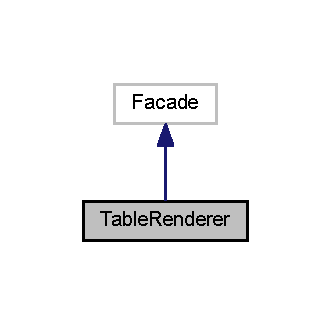
\includegraphics[width=159pt]{classhamburgscleanest_1_1_data_tables_1_1_facades_1_1_table_renderer__coll__graph}
\end{center}
\end{figure}
\subsection*{Static Protected Member Functions}
\begin{DoxyCompactItemize}
\item 
static \hyperlink{classhamburgscleanest_1_1_data_tables_1_1_facades_1_1_table_renderer_a19a808201f41f32f71a0532cb49b450f}{get\+Facade\+Accessor} ()
\end{DoxyCompactItemize}


\subsection{Member Function Documentation}
\mbox{\Hypertarget{classhamburgscleanest_1_1_data_tables_1_1_facades_1_1_table_renderer_a19a808201f41f32f71a0532cb49b450f}\label{classhamburgscleanest_1_1_data_tables_1_1_facades_1_1_table_renderer_a19a808201f41f32f71a0532cb49b450f}} 
\index{hamburgscleanest\+::\+Data\+Tables\+::\+Facades\+::\+Table\+Renderer@{hamburgscleanest\+::\+Data\+Tables\+::\+Facades\+::\+Table\+Renderer}!get\+Facade\+Accessor@{get\+Facade\+Accessor}}
\index{get\+Facade\+Accessor@{get\+Facade\+Accessor}!hamburgscleanest\+::\+Data\+Tables\+::\+Facades\+::\+Table\+Renderer@{hamburgscleanest\+::\+Data\+Tables\+::\+Facades\+::\+Table\+Renderer}}
\subsubsection{\texorpdfstring{get\+Facade\+Accessor()}{getFacadeAccessor()}}
{\footnotesize\ttfamily static get\+Facade\+Accessor (\begin{DoxyParamCaption}{ }\end{DoxyParamCaption})\hspace{0.3cm}{\ttfamily [static]}, {\ttfamily [protected]}}

Get the registered name of the component.

\begin{DoxyReturn}{Returns}
string 
\end{DoxyReturn}


The documentation for this class was generated from the following file\+:\begin{DoxyCompactItemize}
\item 
C\+:/\+Users/chrom/\+\_\+\+P\+A\+G\+E\+S/\+Package\+Dev/packages/hamburgscleanest/\+Data\+Tables/src/\+Facades/Table\+Renderer.\+php\end{DoxyCompactItemize}

\hypertarget{classhamburgscleanest_1_1_data_tables_1_1_helpers_1_1_table_renderer}{}\section{Table\+Renderer Class Reference}
\label{classhamburgscleanest_1_1_data_tables_1_1_helpers_1_1_table_renderer}\index{Table\+Renderer@{Table\+Renderer}}
\subsection*{Public Member Functions}
\begin{DoxyCompactItemize}
\item 
\hyperlink{classhamburgscleanest_1_1_data_tables_1_1_helpers_1_1_table_renderer_aa1cd2b57142fd65141dfcbc7d1a75e98}{open} (? string \$classes=null)
\item 
\hyperlink{classhamburgscleanest_1_1_data_tables_1_1_helpers_1_1_table_renderer_aa69c8bf1f1dcf4e72552efff1fe3e87e}{close} ()
\item 
\hyperlink{classhamburgscleanest_1_1_data_tables_1_1_helpers_1_1_table_renderer_aa0a7cfbdfa3c15180c8e49f27aaac681}{render\+Body} (Collection \$data, array \$columns=\mbox{[}$\,$\mbox{]})
\end{DoxyCompactItemize}


\subsection{Member Function Documentation}
\mbox{\Hypertarget{classhamburgscleanest_1_1_data_tables_1_1_helpers_1_1_table_renderer_aa69c8bf1f1dcf4e72552efff1fe3e87e}\label{classhamburgscleanest_1_1_data_tables_1_1_helpers_1_1_table_renderer_aa69c8bf1f1dcf4e72552efff1fe3e87e}} 
\index{hamburgscleanest\+::\+Data\+Tables\+::\+Helpers\+::\+Table\+Renderer@{hamburgscleanest\+::\+Data\+Tables\+::\+Helpers\+::\+Table\+Renderer}!close@{close}}
\index{close@{close}!hamburgscleanest\+::\+Data\+Tables\+::\+Helpers\+::\+Table\+Renderer@{hamburgscleanest\+::\+Data\+Tables\+::\+Helpers\+::\+Table\+Renderer}}
\subsubsection{\texorpdfstring{close()}{close()}}
{\footnotesize\ttfamily close (\begin{DoxyParamCaption}{ }\end{DoxyParamCaption})}

Closes the table.

\begin{DoxyReturn}{Returns}
string 
\end{DoxyReturn}
\mbox{\Hypertarget{classhamburgscleanest_1_1_data_tables_1_1_helpers_1_1_table_renderer_aa1cd2b57142fd65141dfcbc7d1a75e98}\label{classhamburgscleanest_1_1_data_tables_1_1_helpers_1_1_table_renderer_aa1cd2b57142fd65141dfcbc7d1a75e98}} 
\index{hamburgscleanest\+::\+Data\+Tables\+::\+Helpers\+::\+Table\+Renderer@{hamburgscleanest\+::\+Data\+Tables\+::\+Helpers\+::\+Table\+Renderer}!open@{open}}
\index{open@{open}!hamburgscleanest\+::\+Data\+Tables\+::\+Helpers\+::\+Table\+Renderer@{hamburgscleanest\+::\+Data\+Tables\+::\+Helpers\+::\+Table\+Renderer}}
\subsubsection{\texorpdfstring{open()}{open()}}
{\footnotesize\ttfamily open (\begin{DoxyParamCaption}\item[{? string}]{\$classes = {\ttfamily null} }\end{DoxyParamCaption})}

Starts the table.


\begin{DoxyParams}[1]{Parameters}
null | string & {\em \$classes} & \\
\hline
\end{DoxyParams}
\begin{DoxyReturn}{Returns}
string 
\end{DoxyReturn}
\mbox{\Hypertarget{classhamburgscleanest_1_1_data_tables_1_1_helpers_1_1_table_renderer_aa0a7cfbdfa3c15180c8e49f27aaac681}\label{classhamburgscleanest_1_1_data_tables_1_1_helpers_1_1_table_renderer_aa0a7cfbdfa3c15180c8e49f27aaac681}} 
\index{hamburgscleanest\+::\+Data\+Tables\+::\+Helpers\+::\+Table\+Renderer@{hamburgscleanest\+::\+Data\+Tables\+::\+Helpers\+::\+Table\+Renderer}!render\+Body@{render\+Body}}
\index{render\+Body@{render\+Body}!hamburgscleanest\+::\+Data\+Tables\+::\+Helpers\+::\+Table\+Renderer@{hamburgscleanest\+::\+Data\+Tables\+::\+Helpers\+::\+Table\+Renderer}}
\subsubsection{\texorpdfstring{render\+Body()}{renderBody()}}
{\footnotesize\ttfamily render\+Body (\begin{DoxyParamCaption}\item[{Collection}]{\$data,  }\item[{array}]{\$columns = {\ttfamily \mbox{[}\mbox{]}} }\end{DoxyParamCaption})}

Displays the table body.


\begin{DoxyParams}[1]{Parameters}
Collection & {\em \$data} & \\
\hline
array & {\em \$columns} & \\
\hline
\end{DoxyParams}
\begin{DoxyReturn}{Returns}
string 
\end{DoxyReturn}


The documentation for this class was generated from the following file\+:\begin{DoxyCompactItemize}
\item 
C\+:/\+Users/chrom/\+\_\+\+P\+A\+G\+E\+S/\+Package\+Dev/packages/hamburgscleanest/\+Data\+Tables/src/\+Helpers/Table\+Renderer.\+php\end{DoxyCompactItemize}

\hypertarget{classhamburgscleanest_1_1_data_tables_1_1_models_1_1_header_formatters_1_1_translate_header}{}\section{Translate\+Header Class Reference}
\label{classhamburgscleanest_1_1_data_tables_1_1_models_1_1_header_formatters_1_1_translate_header}\index{Translate\+Header@{Translate\+Header}}


Inheritance diagram for Translate\+Header\+:\nopagebreak
\begin{figure}[H]
\begin{center}
\leavevmode
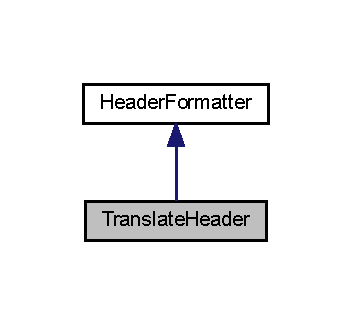
\includegraphics[width=169pt]{classhamburgscleanest_1_1_data_tables_1_1_models_1_1_header_formatters_1_1_translate_header__inherit__graph}
\end{center}
\end{figure}


Collaboration diagram for Translate\+Header\+:\nopagebreak
\begin{figure}[H]
\begin{center}
\leavevmode
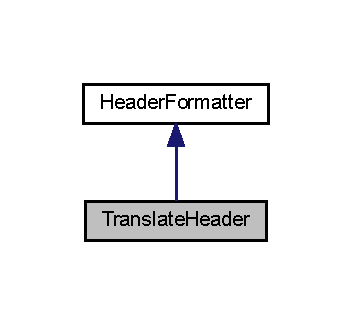
\includegraphics[width=169pt]{classhamburgscleanest_1_1_data_tables_1_1_models_1_1_header_formatters_1_1_translate_header__coll__graph}
\end{center}
\end{figure}
\subsection*{Public Member Functions}
\begin{DoxyCompactItemize}
\item 
\hyperlink{classhamburgscleanest_1_1_data_tables_1_1_models_1_1_header_formatters_1_1_translate_header_acc98a5aed09e4bdbeaa0bd231155a021}{\+\_\+\+\_\+construct} (array \$translations)
\item 
\hyperlink{classhamburgscleanest_1_1_data_tables_1_1_models_1_1_header_formatters_1_1_translate_header_aa5aeddf9c056d9583b29322f75f70f82}{format} (\hyperlink{classhamburgscleanest_1_1_data_tables_1_1_models_1_1_header}{Header} \$header)
\end{DoxyCompactItemize}


\subsection{Constructor \& Destructor Documentation}
\mbox{\Hypertarget{classhamburgscleanest_1_1_data_tables_1_1_models_1_1_header_formatters_1_1_translate_header_acc98a5aed09e4bdbeaa0bd231155a021}\label{classhamburgscleanest_1_1_data_tables_1_1_models_1_1_header_formatters_1_1_translate_header_acc98a5aed09e4bdbeaa0bd231155a021}} 
\index{hamburgscleanest\+::\+Data\+Tables\+::\+Models\+::\+Header\+Formatters\+::\+Translate\+Header@{hamburgscleanest\+::\+Data\+Tables\+::\+Models\+::\+Header\+Formatters\+::\+Translate\+Header}!\+\_\+\+\_\+construct@{\+\_\+\+\_\+construct}}
\index{\+\_\+\+\_\+construct@{\+\_\+\+\_\+construct}!hamburgscleanest\+::\+Data\+Tables\+::\+Models\+::\+Header\+Formatters\+::\+Translate\+Header@{hamburgscleanest\+::\+Data\+Tables\+::\+Models\+::\+Header\+Formatters\+::\+Translate\+Header}}
\subsubsection{\texorpdfstring{\+\_\+\+\_\+construct()}{\_\_construct()}}
{\footnotesize\ttfamily \+\_\+\+\_\+construct (\begin{DoxyParamCaption}\item[{array}]{\$translations }\end{DoxyParamCaption})}

Translatable\+Header constructor. 
\begin{DoxyParams}[1]{Parameters}
array & {\em \$translations} & \\
\hline
\end{DoxyParams}


\subsection{Member Function Documentation}
\mbox{\Hypertarget{classhamburgscleanest_1_1_data_tables_1_1_models_1_1_header_formatters_1_1_translate_header_aa5aeddf9c056d9583b29322f75f70f82}\label{classhamburgscleanest_1_1_data_tables_1_1_models_1_1_header_formatters_1_1_translate_header_aa5aeddf9c056d9583b29322f75f70f82}} 
\index{hamburgscleanest\+::\+Data\+Tables\+::\+Models\+::\+Header\+Formatters\+::\+Translate\+Header@{hamburgscleanest\+::\+Data\+Tables\+::\+Models\+::\+Header\+Formatters\+::\+Translate\+Header}!format@{format}}
\index{format@{format}!hamburgscleanest\+::\+Data\+Tables\+::\+Models\+::\+Header\+Formatters\+::\+Translate\+Header@{hamburgscleanest\+::\+Data\+Tables\+::\+Models\+::\+Header\+Formatters\+::\+Translate\+Header}}
\subsubsection{\texorpdfstring{format()}{format()}}
{\footnotesize\ttfamily format (\begin{DoxyParamCaption}\item[{\hyperlink{classhamburgscleanest_1_1_data_tables_1_1_models_1_1_header}{Header}}]{\$header }\end{DoxyParamCaption})}

Format the given header. For example add a link to sort by this header/column.


\begin{DoxyParams}[1]{Parameters}
\hyperlink{classhamburgscleanest_1_1_data_tables_1_1_models_1_1_header}{Header} & {\em \$header} & \\
\hline
\end{DoxyParams}


Implements \hyperlink{interfacehamburgscleanest_1_1_data_tables_1_1_interfaces_1_1_header_formatter_aa5aeddf9c056d9583b29322f75f70f82}{Header\+Formatter}.



The documentation for this class was generated from the following file\+:\begin{DoxyCompactItemize}
\item 
C\+:/\+Users/chrom/\+\_\+\+P\+A\+G\+E\+S/\+Package\+Dev/packages/hamburgscleanest/\+Data\+Tables/src/\+Models/\+Header\+Formatters/Translate\+Header.\+php\end{DoxyCompactItemize}

\hypertarget{classhamburgscleanest_1_1_data_tables_1_1_helpers_1_1_url_helper}{}\section{Url\+Helper Class Reference}
\label{classhamburgscleanest_1_1_data_tables_1_1_helpers_1_1_url_helper}\index{Url\+Helper@{Url\+Helper}}
\subsection*{Public Member Functions}
\begin{DoxyCompactItemize}
\item 
\hyperlink{classhamburgscleanest_1_1_data_tables_1_1_helpers_1_1_url_helper_acebf296a22e3b9068b929f030a1d0fcb}{query\+Parameters} ()
\end{DoxyCompactItemize}


\subsection{Member Function Documentation}
\mbox{\Hypertarget{classhamburgscleanest_1_1_data_tables_1_1_helpers_1_1_url_helper_acebf296a22e3b9068b929f030a1d0fcb}\label{classhamburgscleanest_1_1_data_tables_1_1_helpers_1_1_url_helper_acebf296a22e3b9068b929f030a1d0fcb}} 
\index{hamburgscleanest\+::\+Data\+Tables\+::\+Helpers\+::\+Url\+Helper@{hamburgscleanest\+::\+Data\+Tables\+::\+Helpers\+::\+Url\+Helper}!query\+Parameters@{query\+Parameters}}
\index{query\+Parameters@{query\+Parameters}!hamburgscleanest\+::\+Data\+Tables\+::\+Helpers\+::\+Url\+Helper@{hamburgscleanest\+::\+Data\+Tables\+::\+Helpers\+::\+Url\+Helper}}
\subsubsection{\texorpdfstring{query\+Parameters()}{queryParameters()}}
{\footnotesize\ttfamily query\+Parameters (\begin{DoxyParamCaption}{ }\end{DoxyParamCaption})}

Array of all the query parameters for the current request.

\begin{DoxyReturn}{Returns}
array 
\end{DoxyReturn}

\begin{DoxyExceptions}{Exceptions}
{\em } & \\
\hline
\end{DoxyExceptions}


The documentation for this class was generated from the following file\+:\begin{DoxyCompactItemize}
\item 
C\+:/\+Users/chrom/\+\_\+\+P\+A\+G\+E\+S/\+Package\+Dev/packages/hamburgscleanest/\+Data\+Tables/src/\+Helpers/Url\+Helper.\+php\end{DoxyCompactItemize}

\hypertarget{classhamburgscleanest_1_1_data_tables_1_1_facades_1_1_url_helper}{}\section{Url\+Helper Class Reference}
\label{classhamburgscleanest_1_1_data_tables_1_1_facades_1_1_url_helper}\index{Url\+Helper@{Url\+Helper}}


Inheritance diagram for Url\+Helper\+:\nopagebreak
\begin{figure}[H]
\begin{center}
\leavevmode
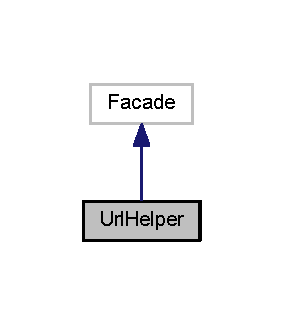
\includegraphics[width=136pt]{classhamburgscleanest_1_1_data_tables_1_1_facades_1_1_url_helper__inherit__graph}
\end{center}
\end{figure}


Collaboration diagram for Url\+Helper\+:\nopagebreak
\begin{figure}[H]
\begin{center}
\leavevmode
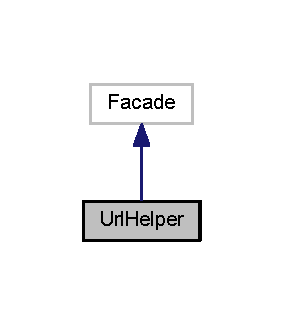
\includegraphics[width=136pt]{classhamburgscleanest_1_1_data_tables_1_1_facades_1_1_url_helper__coll__graph}
\end{center}
\end{figure}
\subsection*{Static Protected Member Functions}
\begin{DoxyCompactItemize}
\item 
static \hyperlink{classhamburgscleanest_1_1_data_tables_1_1_facades_1_1_url_helper_a19a808201f41f32f71a0532cb49b450f}{get\+Facade\+Accessor} ()
\end{DoxyCompactItemize}


\subsection{Member Function Documentation}
\mbox{\Hypertarget{classhamburgscleanest_1_1_data_tables_1_1_facades_1_1_url_helper_a19a808201f41f32f71a0532cb49b450f}\label{classhamburgscleanest_1_1_data_tables_1_1_facades_1_1_url_helper_a19a808201f41f32f71a0532cb49b450f}} 
\index{hamburgscleanest\+::\+Data\+Tables\+::\+Facades\+::\+Url\+Helper@{hamburgscleanest\+::\+Data\+Tables\+::\+Facades\+::\+Url\+Helper}!get\+Facade\+Accessor@{get\+Facade\+Accessor}}
\index{get\+Facade\+Accessor@{get\+Facade\+Accessor}!hamburgscleanest\+::\+Data\+Tables\+::\+Facades\+::\+Url\+Helper@{hamburgscleanest\+::\+Data\+Tables\+::\+Facades\+::\+Url\+Helper}}
\subsubsection{\texorpdfstring{get\+Facade\+Accessor()}{getFacadeAccessor()}}
{\footnotesize\ttfamily static get\+Facade\+Accessor (\begin{DoxyParamCaption}{ }\end{DoxyParamCaption})\hspace{0.3cm}{\ttfamily [static]}, {\ttfamily [protected]}}

Get the registered name of the component.

\begin{DoxyReturn}{Returns}
string 
\end{DoxyReturn}


The documentation for this class was generated from the following file\+:\begin{DoxyCompactItemize}
\item 
C\+:/\+Users/chrom/\+\_\+\+P\+A\+G\+E\+S/\+Package\+Dev/packages/hamburgscleanest/\+Data\+Tables/src/\+Facades/Url\+Helper.\+php\end{DoxyCompactItemize}

%--- End generated contents ---

% Index
\backmatter
\newpage
\phantomsection
\clearemptydoublepage
\addcontentsline{toc}{chapter}{Index}
\printindex

\end{document}
